\documentclass[12pt,article,twosided]{memoir}
%% ::: Memoir class options for page size
%% ::: * the STOCK SIZE is LETTER
%% ::: * the TRIMMED SIZE is 6 x 9
\setlrmarginsandblock{1.25in}{*}{1}
\setulmarginsandblock{1.75in}{*}{1}
\setheadfoot{0.55in}{1in}
\checkandfixthelayout

\usepackage{polyglossia}
\setdefaultlanguage{english}
\setotherlanguage{sanskrit}
\setotherlanguage{tamil}
\setotherlanguage{telugu}
\setotherlanguage{kannada}
\setotherlanguage{malayalam}
\defaultfontfeatures{Mapping=tex-text}
\setmainfont[Numbers={Proportional},SmallCapsFont={TeX Gyre Termes},SmallCapsFeatures={Letters=SmallCaps,Numbers=Lining}]{IndUni-T}
\newfontfamily\tamilfont[Script=Tamil]{AksharUnicodeRegular}
\newfontfamily\sanskritfont[Script=Devanagari]{Jaini}
\newfontfamily\greekfont[Script=Greek]{GFS Porson}
\usepackage[shortcuts]{extdash}
\usepackage{tikz}
\usetikzlibrary{backgrounds, matrix, positioning, fadings, through}
\usepackage{pgf}
\usepackage{tipa}
\usepackage{amssymb}
\usepackage{fontawesome5}
\usepackage{totcount}
\usepackage{calc}
\usepackage{natbib}
	\bibpunct[: ]{(}{)}{; }{a}{ }{,}
\usepackage{xcolor}
\definecolor{Nesarlink}{HTML}{f6820b}
\definecolor{Nesarlinkdark}{HTML}{8a4b0b}
\definecolor{Nesarlinklight}{HTML}{fff0e0}
\usepackage{catchfile}
\usepackage{graphicx,graphbox}
\graphicspath{{images/}}
\usepackage{ragged2e}
\usepackage{tabularx}
\usepackage{changepage}
\usepackage{trimspaces}
\usepackage{framed}
\usepackage[most,breakable]{tcolorbox}
\usepackage[bottom,marginal,multiple]{footmisc}
\def\changemargin#1#2{\list{}{\rightmargin#2\leftmargin#1}\item[]}
\let\endchangemargin=\endlist 
\makeatletter
\renewcommand\@makefntext[1]{%
  \par \parindent=\z@ \noindent
  \llap{\@thefnmark.\quad}%
  {\addfontfeatures{Numbers=Lining}#1}%
}
\ExplSyntaxOn
\cs_set_nopar:Nn{\polyglossia@lang@frenchspacing:n}{\frenchspacing}
\ExplSyntaxOff
\CatchFileDef\slug{metadata/metadata-identifier.tex}{}
\CatchFileDef\doi{metadata/metadata-doi.tex}{}
\newcommand\Ndates{%
\IfFileExists{metadata/metadata-dates-submission.tex}{%
submitted \input{metadata/metadata-dates-submission.tex} {\fontspec{Noto Sans Math}⧫}}{}%
\IfFileExists{metadata/metadata-dates-acceptance.tex}{%
accepted \input{metadata/metadata-dates-acceptance.tex} {\fontspec{Noto Sans Math}⧫}}{}%
\IfFileExists{metadata/metadata-dates-publication.tex}{%
published December 8, 2024}{}
}
% TITLE COMMANDS:
% Ntitle produces Title (no subtitle)
\CatchFileDef\Ntitle{metadata/metadata-title.tex}{}
\title{\protect\trim{\Ntitle}}
% Ntitles produces Title: Subtitle
\newcommand{\Ntitles}{%
\IfFileExists{metadata/metadata-subtitle.tex}{%
{\trim{Meat Matters}}: Meat Matters}{%
Meat Matters}}
\CatchFileDef\citation{metadata/metadata-citation.tex}{}
\makeatother
\def\trim#1{\ignorespaces#1\unskip}
\newcommand{\Nyear}{\trim{2022}}
\newcommand{\Nauthor}{\trim{Jonathan Peterson}}
\author{\protect\Nauthor}
\newcommand{\article}{\trim{1}}
\newcommand{\iy}{\trim{1 (2024): 33–\total{page}.}}
\makeatother
\newcommand{\oldnums}[1]{{\fontspec[Numbers={Proportional,OldStyle}]{TeX Gyre TermesX}#1}}
\newcommand{\oldnumsbold}[1]{{\fontspec[Numbers={Proportional,OldStyle}]{TeX Gyre TermesX}\textbf{#1}}}
\setsecnumformat{\csname #1secnumformat\endcsname}
\newcommand\sectionsecnumformat{\oldnumsbold{\thesection}\quad }
\newcommand\onpage{\oldnums{\thepage}}
\newcommand{\bLozenge}{\mathbin{\blacklozenge}}

\regtotcounter{page}

% Button for CC 4.0 BY
\newcommand{\ccbylicenseButton}{%
\href{https://creativecommons.org/licenses/by/4.0/}{
\includegraphics[align=t,width=2cm]{byNesar.png}}}
% Link to journal
\newcommand{\journallink}{%
\expandafter\url\expandafter{https://nesarjournal.org/articles/\expandafter\slug}}
% Link to DOI
\newcommand{\doilink}{%
DOI: \expandafter\href\expandafter{https://doi.org/\expandafter\doi}{\doi}}
% Issue.Article (Year)
%\newcommand{\iay}{%
%\fontspec[Numbers={Proportional,OldStyle}]{TeX Gyre TermesX}issue \issue, article \article\ (\Nyear)}
% Journal logo and link
\newcommand{\brand}{%

\includegraphics[width=0.5cm,align=c]{logoNesardark.png} \hspace{0.25em} \href{https://nesarjournal.org}{\color{Nesarlinkdark}{\emph{New Explorations in South Asia Research}}}}
% Short author name (small caps, last name)
\newcommand{\shauthor}{\textsc{steinschneider}}
\newcommand\picon[1]{\raisebox{0ex}{\footnotesize{\fontspec{Printers Ornaments One}#1}}}

\makepagestyle{firstpage}
\makeevenfoot{firstpage}{\footnotesize\begin{tabular}[b]{p{5in}}%
© \theauthor\ – \emph{New Explorations in South Asia Research} \iy \\ %{\tiny\fontspec{Noto Sans Math}⧫}
\Ndates\\
\journallink\\
\doilink\end{tabular}}{}{\ccbylicenseButton\vfill}
\makeoddfoot{firstpage}{\footnotesize\begin{tabular}[b]{p{5in}}%
© \theauthor\ – \emph{New Explorations in South Asia Research} \iy \\% {\tiny\fontspec{Noto Sans Math}⧫} 
\Ndates\\
\journallink\\
\doilink\end{tabular}}{}{\ccbylicenseButton\vfill}

\makepagestyle{finalpage}
\makeevenfoot{finalpage}{}{}{}
\makeoddfoot{finalpage}{}{}{}
\makeevenhead{finalpage}{}{}{\onpage}
\makeoddhead{finalpage}{\onpage}{}{}

\captionnamefont{\footnotesize}
\captiontitlefont{\footnotesize}

\newcommand{\footer}{%
\begingroup\vfill\vspace{4ex}\noindent\begin{minipage}[t]{0.3\textwidth}
\noindent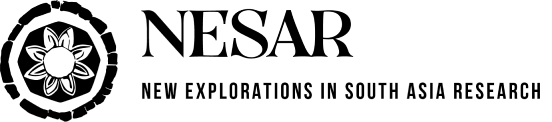
\includegraphics[align=t,width=0.975\textwidth]{logo-wordmark.png}\\[1ex]
\resizebox{0.975\textwidth}{!}{\href{https://nesarjournal.org}{\color{Nesarlinkdark}{\texttt{https://nesarjournal.org}}}}
\end{minipage}\hfill
\begin{minipage}[t]{0.6\textwidth}
\footnotesize\raggedright\noindent{}\citation
\end{minipage}\endgroup}

\createmark{section}{both}{nonumber}{}{}
\nouppercaseheads
\makepagestyle{nesar}
\makeevenhead{nesar}{}{}{\color{Nesarlinkdark}{\thetitle \hspace{0.25em} \picon{e} \hspace{0.25em} \onpage}}
\makeoddfoot{nesar}{\brand\ \iy }{}{}
\makeevenfoot{nesar}{}{}{}
\makeoddhead{nesar}{\color{Nesarlinkdark}{\onpage \hspace{0.35em} \reflectbox{\picon{e}} \hspace{0.25em} \shauthor}}{}{}
\newtcolorbox{titlebox}[1][]{
    enhanced,
    boxrule=2pt,
    colframe=Nesarlinkdark!50!black,
    rounded corners,
    fontupper=\rmfamily,
    colback=Nesarlinklight!50!white,
    #1
    }

\newlength\drop
\newcommand*\titleM
  {%
    \begingroup
    \begin{tikzpicture}[remember picture, overlay]
      \path [bottom color = Nesarlink, top color = white, ] (current page.south west) rectangle ([yshift=-5cm]current page.east);   % Adjust the position of the logo.
    \end{tikzpicture}
    \noindent \emph{An offprint from}\bigskip

    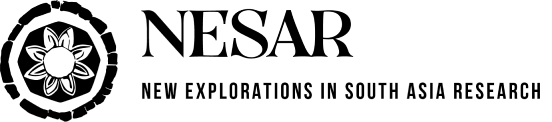
\includegraphics[width=0.65\textwidth]{logo-wordmark.png}
%    \AddToShipoutPictureBG*
%      {%
%        \AtPageLowerLeft
%          {%
%            \includegraphics[width=\paperwidth,height=\paperheight]
%              {example-image-duck}%
%          }%
%      }%
    \setlength\drop{0.15\textheight}%
    \begin{center}%
    \vspace*{\drop}%
    \begin{tikzpicture}[remember picture, overlay]
      \node[inner sep=0pt] (backgroundimage) at ([yshift=-2cm]current page.center) {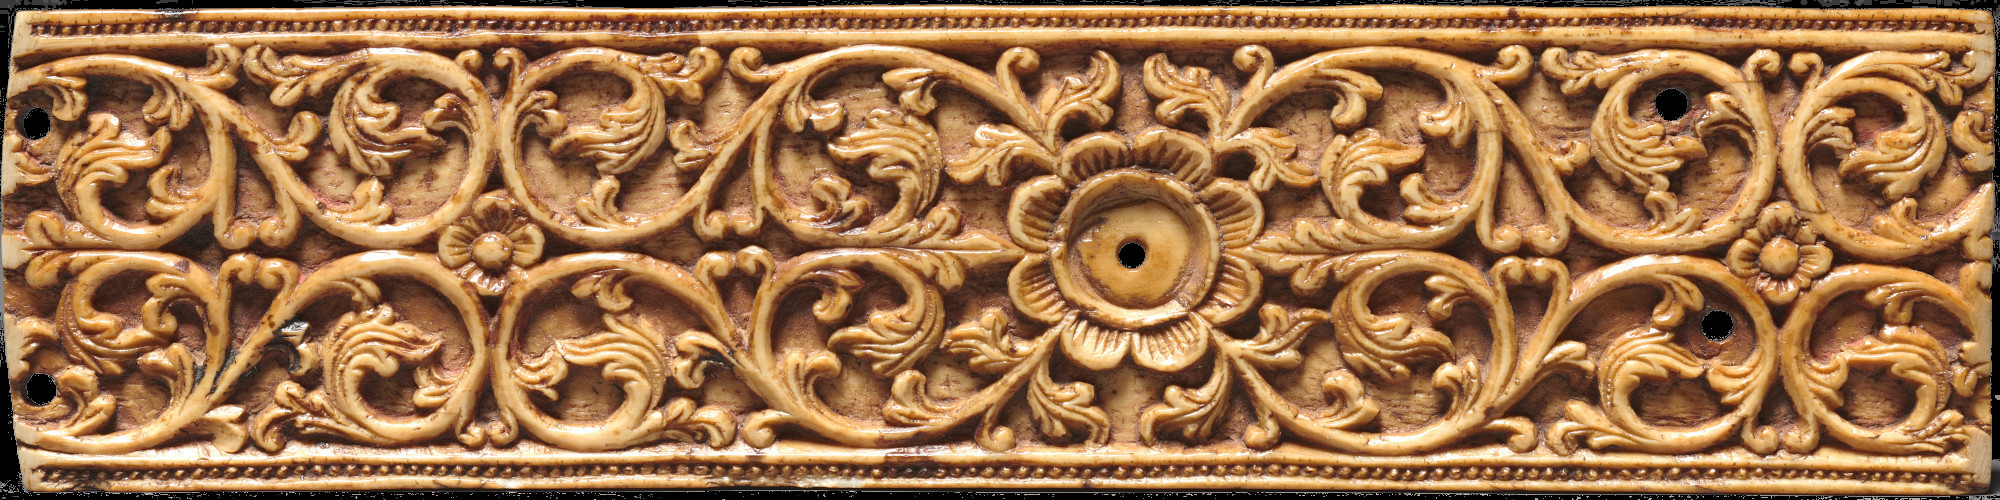
\includegraphics[width=1.2\paperwidth]{ollett-introducing-nesar.jpg}};
      \node[inner sep=0pt] (titlebox) at ([yshift=0.55cm]backgroundimage.north) {\begin{titlebox}\begin{center}\vspace{2ex}%
            \IfFileExists{metadata/metadata-subtitle.tex}{
              {\LARGE\thetitle:\par}\vspace{1ex}
              {\Large\emph{Kolaimaṟuttal} and the Genealogy of Tamil Śaiva Vegetarianism\par}\vspace{2.5ex}
            }{
              {\LARGE\thetitle\par}\vspace{2.5ex}
            }
          {\Large\textit\theauthor\par}\vspace{2ex}
          \end{center}\end{titlebox}};
      \node[inner sep=0pt] (caption) at ([yshift=1cm,xshift=-4.75cm]current page.south east) {\begin{titlebox}[add to width=-6.5cm,fontupper=\linespread{0.75}\selectfont
]%
          {\tiny\raggedright \emph{image source}: Ivory Cover of a Palm-Leaf Manuscript, Sri Lanka, 1600s, Cleveland Museum of Art (via \href{https://commons.wikimedia.org/wiki/File:Ceylon,_17th_century_-_Cover_of_a_Palm-Leaf_Manuscript_-_1992.85_-_Cleveland_Museum_of_Art.tif}{Wikimedia Commons})}%
          \end{titlebox}};

    \end{tikzpicture}
    \vfill
    %{\Large\scshape\press}%
    \end{center}%
    
    \endgroup
  }


\usepackage[linguistics]{forest}
\usepackage{pgfornament}
\usepackage{booktabs,multirow}
\usepackage{wrapfig}
\usepackage{enumitem}
\setlist[itemize]{labelindent=\parindent,itemsep=0.15em,topsep=0pt,leftmargin=\parindent}
\counterwithout{section}{chapter}
\setsecnumdepth{subsubsection}
\maxtocdepth{subsubsection}
\setlength{\cftsectionindent}{1em}
\setlength{\cftsubsectionindent}{1em}
\setlength{\cftsubsubsectionindent}{1em}
\setlength{\parindent}{2em}
\renewcommand{\cftsectionfont}{\bfseries}
\newcommand{\longmark}{{\fontspec{EB Garamond}\raisebox{0.3ex}{ː}\hspace{0.1em}}}
\newcommand{\graph}[1]{{\fontspec{Linux Libertine O}〈#1〉}}
\newcommand{\textgreek}[1]{{\fontspec{GFS Porson}#1}}
\newcommand{\phonet}[1]{{\fontspec{Linux Libertine O}\lbrack#1\rbrack}}
\newcommand{\phonem}[1]{{\fontspec{Linux Libertine O}/#1/}}
\newcommand{\mora}{{\fontspec{GFS Porson}μ}}
\newcommand{\syll}{{\fontspec{GFS Porson}σ}}
\renewcommand{\baselinestretch}{1.1}
\setlength{\RaggedRightParindent}{\parindent}
\frenchspacing
\def\nonfrenchspacing{\frenchspacing}
\AtBeginDocument{\frenchspacing}

\definecolor{formalshade}{rgb}{0.95,0.95,1}
\definecolor{darkblue}{rgb}{0.0, 0.0, 0.55}
\newtcolorbox{pullquote}{
    enhanced,
    boxrule=0pt,
    frame hidden,
    borderline west={2pt}{0pt}{Nesarlinkdark},
    colback=Nesarlinklight,
    sharp corners,
    fontupper=\rmfamily,
    left skip=24pt,
    breakable
    }
\usepackage{xurl}
\usepackage{hyperref}
\hypersetup{pdftitle=\thetitle,
        colorlinks,
        urlcolor=Nesarlink,
        linkcolor=Nesarlink,
        breaklinks=true} 
\usepackage{xurl}
\DeclareRobustCommand{\thinskip}{\hskip 0.16667em\relax}
\def\emdash{—}
\def\d@sh#1#2{\unskip#1\thinskip#2\thinskip\ignorespaces}
\def\Dash{\d@sh\nobreak\emdash}
\def\Ldash{\d@sh\empty{\hbox{\emdash}\nobreak}}
\def\Rdash{\d@sh\nobreak\emdash}

\newcounter{excounter}
\usepackage{hyphenation/nesarhyphenation}
\setcounter{excounter}{1}
\newenvironment{exe}[1]{
\begin{changemargin}{2em}{0em}\noindent\textbf{\theexcounter.\ \ #1}
\end{changemargin}
\begin{changemargin}{4em}{0em}\vspace{-1ex}\noindent\ignorespaces}%
{\end{changemargin}\addtocounter{excounter}{1}}
\widowpenalty10000
\clubpenalty10000

%\usepackage[en]{metre}
%\usepackage{gb4e}
\frenchspacing

\setcounter{page}{33}
\begin{document}
%\RaggedRight

\thispagestyle{empty}
\titleM
\clearpage

\thispagestyle{empty}
\begingroup
\small

\noindent\begin{minipage}[t]{0.8\textwidth}
\noindent\textbf{NEW EXPLORATIONS IN SOUTH ASIA RESEARCH (NESAR)}\smallskip

\noindent An open-access journal of South Asian Studies, founded in 2022.\medskip

\noindent ISSN 2834-3875 \hspace{0.25em} 
\includegraphics[width=0.45cm,align=c]{logoNesar.png} \hspace{0.25em} \url{https://nesarjournal.org}\medskip

\noindent This PDF was generated \today.
\end{minipage}
\begin{minipage}[t]{0.2\textwidth}

\includegraphics[align=t,width=0.5cm]{openaccess.png}
\end{minipage}

\bigskip\bigskip

\noindent\emph{Editorial board}:\smallskip

\noindent\begin{itemize}[itemsep=2pt,parsep=0pt,leftmargin=0.45cm,label={}]
\item Andrew \textsc{OLLETT}, University of Chicago
\item Shubha \textsc{SHANTHAMURTHY}
\item Naresh \textsc{KEERTHI}, Ashoka University
\end{itemize}\medskip

\noindent\emph{Advisory board}:\smallskip

\noindent\begin{itemize}[itemsep=2pt,parsep=0pt,leftmargin=0.45cm,label={}]
\item Diwakar \textsc{ACHARYA}, University of Oxford
\item Richard \textsc{EATON}, University of Arizona
\item Leslie \textsc{ORR}, Concordia University
\item David \textsc{SHULMAN}, Hebrew University of Jerusalem
\item Eva \textsc{WILDEN}, University of Hamburg
\end{itemize}\medskip

\noindent\emph{Principal contact}:\smallskip

\noindent\hspace{0.45cm}Andrew \textsc{OLLETT} (\href{mailto:ollett@uchicago.edu}{\texttt{\color{Nesarlink}ollett@uchicago.edu}})\bigskip\bigskip

\noindent\begin{minipage}[t]{0.48\textwidth}
\begingroup
\tiny\raggedright\noindent
This article is available under a \href{https://creativecommons.org/licenses/by/4.0/}{CC BY 4.0} license. You are free to: 
\begin{itemize}[leftmargin=0.35cm,parsep=0pt,itemsep=0pt]
\item \textbf{Share}: copy and redistribute the material in any medium or format
\item \textbf{Adapt}: remix, transform, and build upon the material for any purpose, even commercially.
\end{itemize}
\noindent under the following terms:
\begin{itemize}[leftmargin=0.35cm,parsep=0pt,itemsep=0pt]
\item \textbf{Attribution}: You must give appropriate credit, provide a link to the license, and indicate if changes were made. You may do so in any reasonable manner, but not in any way that suggests the licensor endorses you or your use.
\item \textbf{No additional restrictions}: You may not apply legal terms or technological measures that legally restrict others from doing anything the license permits.
\end{itemize}\smallskip

\begin{center}

\includegraphics[align=t,width=2cm]{byNesar.png}
\end{center}\smallskip

\tiny\noindent The copyright of this article, as well as all moral rights, rest with the author (\theauthor{}).\vfill

\endgroup
\bigskip
\end{minipage}\hfill
\begin{minipage}[t]{0.48\textwidth}
\begingroup
\tiny
\noindent This PDF file was generated automatically from a source in \href{https://tei-c.org/}{TEI} encoding. The stylesheets used for the transformation are available on \href{https://github.com/nesar-journal/nesar-stylesheets}{this GitHub website}.\medskip

\noindent NESAR uses the \href{https://bombay.indology.info/software/fonts/induni/index.html}{IndUni fonts} designed by John Smith.\medskip

\begin{center}

\includegraphics[width=0.75\textwidth,align=t]{cosas.png}\medskip


\includegraphics[width=0.75\textwidth,align=t]{library.png}
\end{center}\medskip

\noindent NESAR gratefully acknowledges the support of the \href{https://www.lib.uchicago.edu/}{University of Chicago Libraries} and the \href{https://southernasia.uchicago.edu/}{Committee on Southern Asian Studies at the University of Chicago}.\vfill

\endgroup
\end{minipage}
\endgroup
\setcounter{page}{0}
\clearpage

\thispagestyle{firstpage}
\begin{center}
\IfFileExists{metadata/metadata-subtitle.tex}{%
          {\LARGE\thetitle:\par}\vspace{1ex}%
          {\Large\emph{Kolaimaṟuttal} and the Genealogy of Tamil Śaiva Vegetarianism\par}\vspace{1.5ex}%
}{%
          {\LARGE\thetitle\par}\vspace{1.5ex}%
}\bigskip

\begin{tabular}{c}
Andrew Ollett\\[2ex]
{\small\emph{University of Chicago}}\\[1ex]
{\small\href{mailto:ollett@uchicago.edu}{\texttt{ollett@uchicago.edu}}}
\end{tabular}
\end{center}\bigskip

\setlength{\absparsep}{0.5\parskip}
\begin{abstract}
\noindentIn this article, I explore the processes through which Tamil-based Śaivism came to be conceptually equated with the maintenance of a vegetarian diet, a development reflected in the modern Tamil word \emph{caivam} (Skt. \emph{śaiva}), which in colloquial speech primarily signifies lacto-vegetarian cuisine. I contend that although Tamil Śaiva literary sources have long articulated the normativity of vegetarianism, the conflation of Śaiva praxis with plant-based dietary habits likely dates to the late sixteenth and seventeenth centuries. Such, at least, is the picture that emerges from a consideration of the \emph{Kolaimaṟuttal} (\emph{Rejecting Killing}), a brief polemic against animal slaughter likely composed in the then-frontier region of what is now the suburbs of Coimbatore, which emphasizes dietary nonviolence as the quintessential Śaiva virtue and the principal basis for demarcating Śaivism from other religions. A close reading of this hitherto unstudied text suggests that early modern Tamil Śaiva food discourse transformed, at least in part, in response to the emergence of new notions of “self” and “other” in this period, which prompted a corresponding need to rethink the contour and configuration of community boundaries.\medskip

\noindent\textbf{Keywords:} vīraśaiva, madhva, vādirāja tīrtha, vyāsa, desecration, procession, vēdānta, deccan, vyāsantōḷ
\end{abstract}

\pagestyle{nesar}
\clearpage

\begin{KeepFromToc}
  {\small 
  \tableofcontents 
}
\end{KeepFromToc}\bigskip



\raggedbottom
      
\section{Introduction}
      Early in May 1911, the residents of Kolhapur braced for a riot. The city’s Vīraśaivas planned to celebrate the arrival of a prominent monastic leader with a procession. Anticipating backlash, organizers asked Kolhapur’s nominal ruler, Chhatrapati Rajarshi Shahu (descendent of the Maratha leader Shivaji Bhonsle), to personally approve the event. Shahu later recalled in his memoirs that Brahmans in the city “threatened a breach of the peace” were the procession to take place.\footnote{%
\hyperref[Latthe1924]{Latthe} (\hyperref[Latthe1924]{1924}: vol. 2, 345).
}
 They objected not to the arrival of a prominent religious figure, or even to using city streets as a stage for Vīraśaiva piety. Kolhapur’s Brahmans objected to a specific processional object  \Dash  the severed arm of Vyāsa, fabled author of the \emph{Mahābhārata}. Made of bundled rags or gnarled wood, an effigy of Vyāsa’s severed arm  \Dash  known in Kannada simply as \emph{Vyāsantōḷ} (Vyāsa’s arm)  \Dash  would dangle atop a tall pole alongside cymbals, streamers, and a flag decorated with the image of Śiva’s bull, Nandin. During the procession, devotees would hoist the pole aloft while dancing and singing. Some might even swing at Vyāsa’s arm with sticks or swords, reenacting an event from Purāṇic lore when Nandin lopped off Vyāsa’s arm in a fit of pious rage.


Vyāsa’s severed arm had sparked violence elsewhere in the Deccan. There were riots in Bellubbi in 1882, and the \emph{Gazetteer of the Bombay Presidency} reported in 1884 that “many lives were lost” during a conflict in Dharwad a few decades earlier.\footnote{%
\hyperref[Gazetteer]{\emph{Gazetteer}} (1884), pp. 229–230.
}
 “Formerly riots were of constant occurrence,” the \emph{Gazetteer} reads. “The parading of Vyāsa’s hand was forbidden, but in outlying villages the practice is still kept up.”\footnote{%
\hyperref[Gazetteer]{\emph{Gazetteer}} (1884), p. 229.
}
 Vyāsa’s arm may have put parade-goers and passersby at risk, but it seems to have been especially dangerous for organizers. In 1830, at the request of Brahmans in the western reaches of the Mysore state, Krishnaraja Wodeyar III ordered the execution of two Vīraśaiva leaders for organizing a Vyāsa procession.\footnote{%
Wodeyar’s dispensation was found in the library of the Sringeri Śāṅkara \emph{maṭha} at Koodli (near Channagiri) in 1945. Collectors deduced that Wodeyar sent a copy of the decree to Brahmans at the \emph{maṭha} because they petitioned the court to intervene in the procession. Doing so may have endeared Wodeyar to the region’s Mādhva and Smārta Brahmans at a moment when their support was vital to securing Mysore’s power over western Karnataka. It is unclear whether a copy of the document was also sent to the Akṣobhyatīrtha Mādhva \emph{maṭha} in Koodli. See sannad no. 3 in the “Sannads of the Mysore King Mummadi Krishnaraja Wodeyar,” in \hyperref[ARMAD]{\emph{Annual Report}} (1946).
}
 Despite the potential for bloodshed, Shahu approved the parade in Kolhapur and promised his royal marching band as a token of support.


The controversy about Vyāsa’s body in the nineteenth and twentieth centuries was, of course, a product of a particular place and time. The establishment of British common law in the subcontinent, for instance, required that both defenders and challengers of \emph{Vyāsantōḷ} adopt new conceptual and legal categories. But \emph{Vyāsantōḷ} was not an iatrogenic product of colonial law, which is to say that it was not produced by the advent of colonial law itself.\footnote{%
On iatrogenesis and law see \hyperref[Pinney2009]{Pinney} (\hyperref[Pinney2009]{2009}: 29–62).
}
 Though British courts had a hand in refiguring \emph{Vyāsantōḷ} along new conceptual lines, the rhetoric and perhaps even the practice of Vyāsa desecration is evident as early as the late sixteenth century.


This article examines the first known anti-\emph{Vyāsantōḷ} writing, a short Sanskrit poem titled \emph{Praising Vyāsa, Condemning the Apostates} (\emph{{Pāṣaṇḍakhaṇḍanavyāsastōtra}}).\footnote{%
Elsewhere, Vādirāja writes that Buddhists, Jains, and Vīraśaivas  \Dash  the \emph{pāṣaṇḍa}s  \Dash  once accepted, but ultimately rejected, the authority of the Vedas. “Apostate” is closer to this understanding than the more commonly translated “heretic.” See \hyperref[Peterson2023]{Peterson} (\hyperref[Peterson2023]{2023}).
}
 Written by Vādirāja Tīrtha (ca. 1550–1610), an influential poet, scholar, and proselyte of Madhva’s dualist Vedānta, \emph{Praising Vyāsa} provides a starting point for not only plotting the murky history of a particular controversy, but also for rethinking prehistories of religious conflict to include textual polemics and philological disputes.


By invoking the language of religious conflict, I am, of course, thinking of Christopher Bayly and his work on riots in late precolonial and early colonial north India.\footnote{%
\hyperref[Bayly1985]{Bayly 1985}.
}
 Bayly was working against at least two accounts of conflict in the subcontinent. The first was only “dimly aware” of religious violence prior to the rise of colonial commercial power, and the second, while acknowledging the fact of precolonial religious violence, nevertheless maintained that its “quality and incidence” changed dramatically after 1860. Bayly advanced a position of continuity, in which moments of religious conflict in the late nineteenth century are thought to have analogues in the early colonial period. These earlier moments were linked not to religious revivalism or civilizational clashes, Bayly suggested, but to localized shifts of resources and power. Bayly’s work has invited nuancing and criticism since it was written in 1985, but few have challenged the way Bayly consigned texts and their interpretation to little more than symbolic outgrowths or second-order effects of politics and economy.\footnote{%
For instance, see \hyperref[Pandey1990]{Pandey} (\hyperref[Pandey1990]{1990}).
}



This article examines the textual prehistories of what became, in the nineteenth and twentieth centuries, a site of violent agitation and acrimonious litigation. Through a close reading of \emph{Praising Vyāsa} and related texts, I argue several things. First, no \emph{Vyāsantōḷ} text was itself the pretext for conflict. Nor were \emph{Vyāsantōḷ} texts the mere sublimation of strife on the ground. The desecration of Vyāsa’s body and its ceremonial display in city streets in the nineteenth and twentieth centuries emerged from an interplay of text and practice  \Dash  a kind of mimetic loop  \Dash  in which forms of interpretation informed paradigms of performance and vice versa.


The movement between reading, performance, and public spectacle was accelerated in part by Vyāsa’s migration from a fictive figure of epic antiquity to a centerpiece of devotion among Vaiṣṇavas of various orders, and especially among a community of Viṣṇu devotion and Vedānta organized around the figure of Madhva (ca. 1238–1317 \textsc{ce}). Styled as both an emanation of Viṣṇu as well as Madhva’s guru, Vyāsa imparted to Madhva’s writings, and by extension to his dualist Vedānta philosophy, both soteriological and scholastic legitimacy. It is unsurprising, then, that followers of Madhva wrote numerous Vyāsa praise poems and that even the notional desecration of Vyāsa’s body would be interpreted as an affront to the very affective and soteriological core of Madhva’s devotional community.


Whether Vyāsa’s arm was a processional object before the early nineteenth century is unclear. Even its presence in writing before the nineteenth century is fleeting. The second part of this article puts forward a provisional genealogy of \emph{Vyāsantōḷ}. Episodes of divine dismemberment are not uncommon in Sanskrit literature, and the case of Vyāsa’s arm appears to adapt and amplify earlier motifs of “aggressive bodily intervention” seen in Sanskrit epics, Śaiva Purāṇas, and Vīraśaiva didactic texts.\footnote{%
See Jesse Pruitt’s forthcoming work on the \emph{{Śivadharmōttara}}.
}
 The closest parallel to the amputation of Vyāsa’s arm is its paralysis. I look at several examples of Vyāsa’s monoplegia. The first is from the \emph{{Skanda Purāṇa}}, where Vyāsa confronts Śiva with a sermon about Viṣṇu’s superiority and is paralyzed in turn. Similar moments of paralysis are found in earlier texts, including the \emph{Mahābhārata} and the \emph{{Śivadharmōttara}}. Yet these cases of paralysis are usually reversed and are thus symbolically distinct from the permanent dismemberment of \emph{{Vyāsantōḷ}}. Earlier motifs of paralysis appear to have undergone a consequential intensification in the fourteenth and fifteenth centuries. This is apparent, for instance, in Vīraśaiva didactic texts like Śivayogin’s (ca. fourteenth century \textsc{ce}) \emph{{Siddhāntaśikhāmaṇi}} and its early-modern commentaries, where Śiva’s slanderers are met with more egregious forms of bodily harm. 


Here I must emphasize that these were textual dictates, and that the gap between text and life on the ground  \Dash  at least where they concern violence against those who challenge Vīraśaivas and their institutions  \Dash  appears to have been vast indeed. When Vādirāja wrote \emph{Praising Vyāsa} in the late sixteenth century, swaths of his home in western Karnataka were controlled by a powerful Vīraśaiva ruling family. Rather than curse or kill critics of Vīraśaivas, the Nāyakas of western Karnataka lavished them, including Vādirāja, with royal largesse.


The sources I present here show Vyāsa’s arm as a surrogate for several things simultaneously. By the end of the sixteenth century, it had become a token of sectarian triumph, where Śiva could win over the most ardent devotee of Viṣṇu, even if only by force. For Vādirāja, the desecration of Vyāsa was both an egregious textual misinterpretation and an unforgivable attack on the legitimacy of Madhva and his Vedānta. What I do not touch on here, but which hangs over the entire \emph{Vyāsantōḷ} controversy, is caste. Vyāsa’s venerated position among Vaiṣṇava and Śaiva Brahmans alike would have rendered his desecration a potent symbol of anti-caste agitation. And with the rise of the Vīraśaiva ruling family of western Karnataka, the flagrant desecration of an exemplar of caste elitism may have marked a turn in subaltern political power and its symbolic expression.


I conclude with a perfunctory examination of \emph{Vyāsantōḷ}’s juridical life, which allows me to highlight at least two avenues of further research. The first might be a new direction in the study of the \emph{Mahābhārata}. While anthropologists and historians have noted the \emph{Mahābhārata}’s various localizations and retellings, Sanskrit epics as points of sectarian, caste, and legal conflict are largely unstudied. Second are the legal afterlives of premodern Sanskrit polemics in colonial India. I have in mind both the direct and indirect ways that precolonial Sanskrit disputes, especially over issues of inheritance, property, marriage, temple access, procession, and so on, shaped legal discussions in the nineteenth and twentieth centuries. But early modern Sanskrit polemics about \emph{Vyāsantōḷ} are interesting not because of their influence on later legal debates, but because they appear to have had no influence at all. Though Vyāsa’s body remained a source of outrage, modes of what we might call “philological containment”  \Dash  erudite (if still vitriolic) Sanskrit polemics as a strategy of conflict management  \Dash  seem to have given way to political violence and courtly machinations.

\section{Conjuring the Image of Vyāsa}
      Vyāsa was probably never a real person, though some of the deeds ascribed to him may have been the work of many people over many centuries.\footnote{%
Later Purāṇas speak of as many as eighteen Vyāsas. See \emph{{Viṣṇupurāṇa}} 3.3.9.
}
 Yet when Vādirāja wrote \emph{Praising Vyāsa, Condemning the Apostates} in the late-sixteenth century, Vyāsa had long been transformed into a god. To do justice to his divinization alone would warrant a separate study.\footnote{%
The figure of Vyāsa has accumulated a considerable scholarship. A study of his divinization alone would include \hyperref[Shembavnekar1947]{Shembavnekar} (\hyperref[Shembavnekar1947]{1947}), who showed that “Vyāsa had nothing to do with the four Vedas.” It would include volumes written about Vyāsa in the field of \emph{Mahābhārata} studies, such as \hyperref[Sullivan1999]{Sullivan} (\hyperref[Sullivan1999]{1999}) and also studies on specific chapters and sections of the \emph{Mahābhārata}. Grünendahl (\hyperref[Gruenendahl1989]{1989} and \hyperref[Gruenendahl2002]{2002}, and \hyperref[Gruenendahl1997]{Grünendahl and Schreiner 1997}) for instance, describes how Vyāsa became an “emanation of Nārāyaṇa,” and the scholarship of \hyperref[Biardeau2002]{Biardeau} (\hyperref[Biardeau2002]{2002}), \hyperref[Hiltebeitel2005]{Hiltebeitel} (\hyperref[Hiltebeitel2005]{2005}), and others has convincingly shown the \emph{{Nārāyaṇīyaparvan}} to be a later feature of the epic and to reflect the interests of new cults of Viṣṇu worship in the first centuries \textsc{ce}. Such a study would also include work on Vyāsa in the Purāṇas, like \hyperref[Saindon20042005]{Saindon} (\hyperref[Saindon20042005]{2004–2005}) and \hyperref[Bisschop2021]{Bisschop} (\hyperref[Bisschop2021]{2021}). 
}
 My starting point here, however, is Vyāsa after apotheosis.


Vyāsa’s identity as Viṣṇu had not only been a given for Madhva and his early followers; it was vital for establishing Madhva’s legitimacy as a Vedānta commentator. Vyāsa plays an especially prominent role in Madhva’s \emph{Determining the Ultimate Aim of the Mahābhārata} (\emph{{Mahābhāratatātparyanirṇaya}}), which emplots the tenets of Madhva’s Vedānta within the narrative arcs of the \emph{Mahābhārata} and the \emph{Rāmāyaṇa}. In addition to peppering the commentary with his own Vyāsa encomia, Madhva dutifully reiterates the few existing \emph{Mahābhārata} verses that equate Vyāsa with God. “You should know Kr̥ṣṇa Dvaipāyana Vyāsa as the Lord Nārāyaṇa,” Madhva repeats.\footnote{%
See Madhva’s \emph{{Mahābhāratatātparyanirṇaya}} (ed. \hyperref[Madhva2009]{Gōvindācārya}), v. 2.41, and \emph{Mahābhārata} 12.334.9 (ed. \hyperref[MBh]{Sukthankar and Belvalkar}):

\vspace{-1.5ex}\begin{quote}\raggedright
      \emph{kr̥ṣṇadvaipāyanaṁ vyāsaṁ viddhi nārāyaṇaṁ prabhum}\end{quote}\vspace{-1.5ex}
      }



One of the “ultimate aims” Madhva wanted his readers to take from his \emph{Mahābhārata} commentary was that Viṣṇu-as-Vyāsa sanctioned both Madhva’s divine nature and his dualist Vedānta project. In the commentary’s second chapter, for instance, Vyāsa announces Madhva as an incarnation of the god Vāyu. Citing a verse from the Bhaviṣyatparvan, but which is not found in any recension of the text, Vyāsa proclaims:

\begin{pullquote}\raggedright
      \emph{tasyāṅgaṁ prathamaṁ vāyuḥ prādurbhāvatrayānvitaḥ}\\
\emph{prathamō hanumān nāma dvitīyō bhīma ēva ca}

\emph{pūrṇaprajñas tr̥tīyas tu bhagavatkāryasādhakaḥ}\\
\emph{trētādyēṣu yugēṣv ēṣa saṁbhūtaḥ kēśavājñayā}
\end{pullquote}
      
\begin{pullquote}


	
	      The first subsidiary of Viṣṇu is Vāyu,\\
	      who has three worldly manifestations.\\
	      The first is called Hanumān, the second, Bhīma.\\
	      But the third is Madhva, fulfiller of God’s deeds.\\
	      At Viṣṇu’s decree, Vāyu has appeared in the first three epochs.\footnotemark{}
	    \\


\medskip\hfill\begin{minipage}{0.9\textwidth}\small\hfill
Madhva, \emph{{Mahābhāratatātparyanirṇaya}} (ed. \hyperref[Madhva2009]{Gōvindācārya}, vv. 2.124–125, pp. 88–89)\end{minipage}\hspace{2em}
\end{pullquote}\footnotetext{Madhva says the verse is from the Bhaviṣyatparvan of the \emph{{Harivaṁśa}}, but it is probably one of his own compositions. For more on Madhva’s untraceable sources, see Mesquita (\hyperref[Mesquita2000]{2000}, \hyperref[Mesquita2008]{2008}).
}

The clamor that Madhva’s messianic self-styling caused in the centuries after his death obscured the messenger himself. Strictly speaking, Madhva did not announce his own divine nature, Vyāsa did. As an emanation of Viṣṇu, Vyāsa transformed Madhva’s unprecedented claim of his own divinity into a scriptural dictate. To deny Vyāsa’s declaration of Madhva’s divine nature, in other words, would be tantamount to denying the authority of the \emph{Mahābhārata} itself.


Elsewhere, Madhva invokes Vyāsa as his guru, which allowed for elaborate narratives about Madhva’s connection to Vyāsa in early hagiographies. Nārāyaṇa Paṇḍita (ca. fourteenth century \textsc{ce}), for instance, devotes the seventh chapter of his \emph{{Śrīmadhvavijaya}} to narrating Madhva’s visit to Vyāsa’s Himalayan hermitage. Daniel Sheridan has shown how this episode connects Madhva and his writings to Vyāsa by asserting a direct student-teacher relation.\footnote{%
\hyperref[Sheridan1992]{Sheridan} (\hyperref[Sheridan1992]{1992}).
}
 But this didactic connection is, by measure of verse, an utterly minor feature of Madhva’s life story. Far more significant, both as a narrative fact and for their influence on devotional practice, are the dozens of verses Nārāyaṇa devotes to Madhva’s inner monologue upon seeing Vyāsa in the flesh.\footnote{%
Concealed from ordinary people during the Kali Age, Vyāsa nevertheless welcomes Madhva’s mind and eyes (\emph{cetōnayanābhinandana}). Nārāyaṇa likens Vyāsa’s disappearance from the vision of ordinary people in the Kali Age to the disappearance of the sun at night (Nārāyaṇa Paṇḍita, \emph{{Śrīmadhvavijaya}} [ed. \hyperref[NarayanaPandita2017]{Gōvindācārya}] v. 7.22).:

\vspace{-1.5ex}\begin{quote}\raggedright
      \emph{adhunā kalikālavr̥ttayē savitēva kṣaṇadānuvr̥ttayē}\\
\emph{janadr̥gviṣayatvam atyajad bhagavān āśramam āvasann imam}\end{quote}\vspace{-1.5ex}
      }
 “Even though Madhva had always seen Vyāsa in his pure, lotus heart,” Nārāyaṇa writes, “upon seeing Vyāsa again anew, Madhva became wonderstruck and thought the following to himself.”\footnote{%
Nārāyaṇa Paṇḍita, \emph{{Śrīmadhvavijaya}} (ed. \hyperref[NarayanaPandita2017]{Gōvindācārya} v. 7.17):

\vspace{-1.5ex}\begin{quote}\raggedright
      \emph{nijahr̥tkamalē ’tinirmalē satataṁ sādhu niśāmayann api}\\
\emph{avalōkya punaḥ punar navaṁ tam asau vismita ity acintayat}\end{quote}\vspace{-1.5ex}
      }
 The next thirty verses describe Madhva’s cascade of observations about Vyāsa’s body, from the dust on Vyāsa’s feet to the matted hair on his head. Madhva’s life story, in other words, takes a sharp detour into Vyāsa encomia. About Vyāsa’s feet, for instance, Madhva thinks to himself:

\begin{pullquote}\raggedright
      \emph{kamalākamalāsanānilair vihagāhīndraśivēndrapūrvakaiḥ}\\
\emph{padapadmarajō ’sya dhāritaṁ śirasā hanta vahāmy ahaṁ muhuḥ}\\
\emph{praṇamāmi padadvayaṁ vibhōr dhvajavajrāṅkuśapadmacihnavat}\\
\emph{nijamānasarāgapīḍanād aruṇībhūtam ivāruṇaṁ svayam}\\
\emph{nanu kēvalam ēva vaiṣṇavaṁ śritavantaḥ padam ātmarōciṣā}\\
\emph{tamasō ’py ubhayasya nāśakā vijayantē nakharā navaṁ ravim}\\
\emph{sukumāratarāṅgulīmatōḥ padayōr asya nigūḍhagulphayōḥ}\\
\emph{upamānam ahō na dr̥śyatē kavivaryair itarētaraṁ vinā}
\end{pullquote}
      
\begin{pullquote}
Wow! I have the dust of Vyāsa’s lotus feet on my head, the same dust that Lakṣmī, Brahmā, Vāyu, Garuḍa, Śeṣa, Śiva, and Indra once had on theirs. I bow to the lord’s two feet, which are marked with Viṣṇu’s banner, lightning bolt, goad, and lotus. Though naturally ruddy, his two feet appear to have become even more so after beating back the mental passions of his followers. His toenails, which have taken refuge at Viṣṇu’s feet, destroy two kinds of darkness (internal and external) with their luster, and thus surpass even the sun at daybreak. Except for one or the other foot, the best poets fail to find an adequate analogy for Vyāsa’s two feet, which have the most delicate toes and concealed ankles.\footnotemark{}


\medskip\hfill\begin{minipage}{0.9\textwidth}\small\hfill
Nārāyaṇa Paṇḍita, \emph{{Śrīmadhvavijaya}} (ed. \hyperref[NarayanaPandita2017]{Gōvindācārya} v. 7.25–28)\end{minipage}\hspace{2em}
\end{pullquote}\footnotetext{The verb \emph{śritavantaḥ} in verse 27 conveys that the toenails are both connected to and have taken refuge at Viṣṇu’s feet, much as a disciple might. The suggestion seems to be that just as the toenails remove darkness and surpass the sunrise in their splendor, so too the disciple  \Dash  in this case, Madhva  \Dash  can do the same. 
}

Madhva’s encounter with Vyāsa allowed Nārāyaṇa to conjure an intimate portrait of Vyāsa’s body in the minds of his readers. It is worth dwelling on this image for a moment. Vyāsa’s legs are “fittingly burly from bottom to top,” and “cause the person who worships him to become the same.”\footnote{%
\hyperref[NarayanaPandita2017]{\emph{ibid.}}, v. 7.29:\setlength{\parindent}{2em}

\vspace{-1.5ex}\begin{quote}\raggedright
      \emph{ucitāṁ gurutāṁ dadhat kramāc chuci tējasvi suvr̥ttam uttamam}\\
\emph{bhajatō ’tra ca bhājayaty adō vibhujaṅghayugalaṁ sarūpatām}\end{quote}\vspace{-1.5ex}
      

\noindent{}“The Lord’s two legs, appearing fittingly burly from bottom to top, are pure, brilliant, well-made, and excellent. They cause the person who worships him to become the same/to attain \emph{mōkṣa}.” The pun here is on \emph{sarūpatā} being a stage of \emph{mōkṣa}, on which reading the legs confer the appropriate \emph{gurutā} according to one’s stage of enlightenment (cf. \emph{{Br̥hadāraṇyaka Upaniṣad}} 5.13.1–4 [ed. \hyperref[Olivelle1998]{Olivelle}], which is echoed later in the \emph{{Bhāgavatapurāṇa}} and elsewhere).
}
 Sitting on a deerskin that shines with the “lovely sheen of sunlight,” Vyāsa possesses a miraculous hue.\footnote{%
\hyperref[NarayanaPandita2017]{\emph{ibid.}}, vv. 7.30–31:\setlength{\parindent}{2em}

\vspace{-1.5ex}\begin{quote}\raggedright
      \emph{acalāsanayōgapaṭṭikā varakakṣyā sakr̥dāptam iṣṭadam}\\
\emph{paritō ’pi hariṁ sphuranty ahō aniśaṁ dhanyatamēti mē matiḥ}

\emph{rucirēṇa varēṇa carmaṇā rucirājadyuticārurōciṣā}\\
\emph{paramōrunitambasaṅginā paramāścaryatayā virājyatē}\end{quote}\vspace{-1.5ex}
      

\noindent{}“A meditation cloth for steady sitting posture, which has the finest hems, shines from all sides upon Hari as Vyāsa, who gives whatever is desired even when approached once  \Dash  that cloth, in my opinion, is the most praiseworthy thing. The resplendent deer skin upon which he sits, which has the lovely sheen of sunlight, makes him appear most miraculous.” Bāṇa used the term \emph{yōgapaṭṭaka} several times in the \emph{{Harṣacarita}}. It means both a meditation cloth and a forged royal document. In his edition of the text, P. V. \hyperref[Kane1918]{Kane} (\hyperref[Kane1918]{1918}: notes, 26) gives the following explanatory verse. From where it comes, I am not sure.

\vspace{-1.5ex}\begin{quote}\raggedright
      \emph{pr̥ṣṭhajānvōḥ samāyoge vastraṁ valayavad dr̥ḍham}\\
\emph{parivēṣṭya yad ūrdhvajñus tiṣṭhēt tad yōgapaṭṭakam}\end{quote}\vspace{-1.5ex}
      }
 His “slender, soft, beautiful lotus belly” contains the whole universe.\footnote{%
\hyperref[NarayanaPandita2017]{\emph{ibid.}}, v. 7.32:\setlength{\parindent}{2em}

\vspace{-1.5ex}\begin{quote}\raggedright
      \emph{tanunimnasunābhiśōbhitē valibhē vārijanābha ādadhē}\\
\emph{pratanāv atisundarē mr̥dāv udarē ’smin jagadaṇḍamaṇḍalam}\end{quote}\vspace{-1.5ex}
      

\noindent{}“He has kept the sphere of the universe in this slender, soft, beautiful lotus belly, which has delicate folds, and which is adorned with a soft, deep navel.”
}
 Nārāyaṇa exploits the ambiguous word division in the phrase \emph{brahma-su-sūtram} to simultaneously tell us that Vyāsa’s chest appears white because of the \emph{upanayana} thread (\emph{brahmasu sūtram}) and that his heart is captivating because it holds the glorious aphorisms about \emph{brahman}, that is, the \emph{{Brahmasūtra}}s (\emph{brahmasusūtra}).\footnote{%
\hyperref[NarayanaPandita2017]{\emph{ibid.}}, vv. 7.33–34:\setlength{\parindent}{2em}

\vspace{-1.5ex}\begin{quote}\raggedright
      \emph{hr̥dayē kr̥tasajjanōdayē suviśālē vimalē manōharē}\\
\emph{ubhayaṁ vahati trayīmayaṁ bhagavān brahmasusūtram uttamam}

\emph{asamē ’nadhikē susādhitē nijatātē ravirāśidīdhiti}\\
\emph{pradadau trijagajjayadhvajaṁ vidhir ētad galasaṅgibhūṣaṇam}\end{quote}\vspace{-1.5ex}
      

\noindent{}“The lord holds the two best Vedic \emph{sūtra}s: One he wears on his broad chest, the other he holds in his expansive heart, which uplifts the righteous. In the case of the [\emph{upanayana}] thread on Brahmans [\emph{brahmasu sūtra}], his chest is white and beautiful, whereas in the case of the glorious aphorisms about \emph{brahman} [i.e., the \emph{{Brahmasūtra}}], his heart is pure and captivating. When Vyāsa proved [through his various compositions] that Viṣṇu is unequaled and unsurpassed, Brahmā gave him this ornament, the \emph{kaustubha} gem, which hangs around his throat as a symbol of his conquest over the three worlds and which shines like a cluster of suns.” The word \emph{susūtra} can be glossed as \emph{śōbhanam sūtram iti susūtram}.
}
 His arms possess soft, ruddy hands that have the marks of Viṣṇu’s discus and conch.\footnote{%
\hyperref[NarayanaPandita2017]{\emph{ibid.}}, vv. 7.35–36:\setlength{\parindent}{2em}

\vspace{-1.5ex}\begin{quote}\raggedright
      \emph{arivārijalakṣaṇōllasatsukumārārūṇapāṇipadmayōḥ}\\
\emph{pr̥thupīvaravr̥ttahastayōr upamāṁ naiva labhāmahē ’nayōḥ}

\emph{bhavatāṁ varatarkamudrayā dyati hastāgram abōdham īśituḥ}\\
\emph{adhijānusamarpitaṁ paraṁ kr̥tabhūyōbhayabhaṅgamaṅgalam}\end{quote}\vspace{-1.5ex}
      

\noindent{}“I cannot find a comparison for these two arms, which have large, brawny, and round forearms, which have lotus-like hands that are soft, ruddy, and resplendent with the marks of Viṣṇu’s discus and conch. Through \emph{jñānamudrā}, the fingers of one hand destroy the ignorance of devotees. The fingers of the other sit atop the knee, auspicious for their part in vanquishing tremendous fear.”
}
 His neck has three auspicious lines, one for each of the Vedas he composed.\footnote{%
\hyperref[NarayanaPandita2017]{\emph{ibid.}}, v. 7.37:\setlength{\parindent}{2em}

\vspace{-1.5ex}\begin{quote}\raggedright
      \emph{satataṁ galatā svataḥ śrutitritayēnēva nikāmam aṅkitaḥ}\\
\emph{suviḍambitakambur īkṣyatē vararēkhātrayavān guror galaḥ}\end{quote}\vspace{-1.5ex}
      

\noindent{}“I see Vyāsa’s neck, which, perfectly resembling a conch shell, has three auspicious lines; the neck, which is clearly marked [or numbered] by the three Vedas that issue forth [from his throat] eternally.”
}
 Vyāsa’s face outshines the light of a thousand beams from a spotless moon, and the appearance of his teeth against his red lips “put to shame a string of new pearls glimmering on ruby facets.”\footnote{%
\hyperref[NarayanaPandita2017]{\emph{ibid.}}, vv. 7.38–39:\setlength{\parindent}{2em}

\vspace{-1.5ex}\begin{quote}\raggedright
      \emph{sakalāstakalaṅkakālimasphuradinduprakarōruvibhramam}\\
\emph{adharīkurutē svaśōbhayā vadanaṁ dēvaśikhāmaṇēr idam}

\emph{aruṇāśmadalāntarōllasannavamuktāvalim asya lañjayēt}\\
\emph{hasataḥ sitadantasantatiḥ paramaśrīr aruṇoṣṭharōciṣaḥ}\end{quote}\vspace{-1.5ex}
      

\noindent{}“By its own splendor, the face of Vyāsa  \Dash  the crown jewel of the gods  \Dash  outshines even the beautiful light from a thousand moon rays blazing brightly after the moon’s spots have been completely removed. Smiling and effulgent with red lips, Vyāsa has a row of the most beautiful white teeth that would put to shame a string of new pearls glimmering on ruby facets.”
}
 His speech, likened to a infinite spring of freshwater, fills the “wells which are the questions posed by thousands of Brahmans.”\footnote{%
\hyperref[NarayanaPandita2017]{\emph{ibid.}}, v. 7.40:\setlength{\parindent}{2em}

\vspace{-1.5ex}\begin{quote}\raggedright
      \emph{dvijavr̥ndakr̥taṁ kutūhalād anuyōgāndhusahasram uttamam}\\
\emph{iyam ēkapadē sarasvatī śrutibhartuḥ paripūrayaty ahō}\end{quote}\vspace{-1.5ex}
      

\noindent{}“Amazing! With a single word, the Lord of Scripture’s riverine speech miraculously fills up thousands of well-like questions posed by scores of Brahmans.”
}
 The Tulasi leaf that sits upon Vyāsa’s ear whispers, “O Lord, please do not let the lotus and other flowers steal my position out of jealousy.”\footnote{%
\hyperref[NarayanaPandita2017]{\emph{ibid.}}, vv. 7.41–42:\setlength{\parindent}{2em}

\vspace{-1.5ex}\begin{quote}\raggedright
      \emph{jalajāyatalōcanasya mām avalōkō ’yam upētya lālayan}\\
\emph{kurutē parirabhya pūritaṁ bhuvanānandakarasmitānvitaḥ}

\emph{upakarṇam amuṣya bhāsitā tulasī mantrayatīva lālitā}\\
\emph{mama nātha padaṁ na matsarāj jalajādyāni hareyur ity alam}\end{quote}\vspace{-1.5ex}
      

\noindent{}“I became fulfilled after this sportive gaze of Vyāsa  \Dash  whose eyes are wide like lotus petals  \Dash  fell to me and embraced me, the gaze accompanied by a smile that makes all sentient beings happy. It is as if the beloved Tulasi leaf that sits just above his ear mutters silently to itself  \Dash  ‘O Lord! Let not the lotus and other flowers steal my position out of jealousy.’”
}
 And after describing his eyebrows and forehead, Madhva thinks about Vyāsa’s miraculous body and its innumerable qualities:\footnote{%
\hyperref[NarayanaPandita2017]{\emph{ibid.}}, vv. 7.43–44:\setlength{\parindent}{2em}

\vspace{-1.5ex}\begin{quote}\raggedright
      \emph{vibhavābhibhavōdbhavādikaṁ bhuvanānāṁ bhuvanaprabhōr bhruvōḥ}\\
\emph{anayōr api dabhravibhramāt sabhavāṁbhōjabhavātmanāṁ bhavēt}

\emph{trijagattilakālikāntarē tilakō ’yaṁ parabhāgam āptavān}\\
\emph{harinīlagirīndramastakasphuṭaśōṇōpalapaṅktisannibhaḥ}\end{quote}\vspace{-1.5ex}
      

\noindent{}“From the slightest quiver of the Lord of Creation’s eyebrows would result the destruction, maintenance, and birth of all existing things, which have as their nature Śiva and Brahmā. This \emph{tilaka}  \Dash  which is indistinguishable from a row of rubies shining resplendent atop a sapphire mountain  \Dash  has attained eminence in the middle of the Ornament of the Three Worlds’ forehead.”
}


\begin{pullquote}\raggedright
      \emph{navam ambudharaṁ viḍambayad varavidyudvalayaṁ jagadgurōḥ}\\
\emph{avalōkya kr̥tārthatām agāṁ sajaṭāmanḍalamanḍanaṁ vapuḥ}

\emph{na ramāpi padāṅgulīlasannakhadhūrājadanantasadguṇān}\\
\emph{gaṇayēd gaṇayanty anārataṁ paramān kō ’sya parō guṇān vadēt}

\emph{na kutūhalitā kutūhalaṁ tanum ēnām avalōkya sadgurōḥ}\\
\emph{sanavāvaraṇāṇḍadarśinō gr̥habuddhyā mama niṣkutūhalam}
\end{pullquote}
      
\begin{pullquote}
I became completely satisfied upon seeing the Lord of the Worlds’ body, which, with its most precious, lightning-bright arm band, resembles a new raincloud, and is festooned with a matted knot of hair. Not even Lakṣmī, despite continuously counting, could keep track of the innumerable, sanctified qualities emanating from just the movement of the toenails of Vyāsa’s feet. Who could possibly describe his virtues?


\medskip\hfill\begin{minipage}{0.9\textwidth}\small\hfill
Nārāyaṇa Paṇḍita, \emph{{Śrīmadhvavijaya}} (ed. \hyperref[NarayanaPandita2017]{Gōvindācārya} vv. 7.45–48)\end{minipage}\hspace{2em}
\end{pullquote}

Simile, metaphor, alliteration, pun, and other poetic devices are key to conjuring Vyāsa’s image in the minds of Nārāyaṇa’s readers. So, too, is the failure of poetic language. Twice Nārāyaṇa stresses that words fail to express Vyāsa’s true glory. Even Lakṣmī cannot fully enumerate the qualities of Vyāsa’s toenails, let alone the totality of his body. How could a poet? Yet later Mādhva poets nevertheless tried. Nārāyaṇa’s \emph{{Vyāsastōtra}} is a precursor for later Vyāsa praise poems. In addition to \emph{Praising Vyāsa, Condemning the Apostates}, several other \emph{{Vyāsastōtra}}s are attributed to Vādirāja, including \emph{Eight Verses to Vyāsa} (\emph{{Vyāsāṣṭaka}}) and \emph{Describing Vyāsa} (\emph{{Vyāsavarṇana}}). Simple but rich compositions, \emph{Eight Verses} and \emph{Describing Vyāsa} appear to have been written for popular consumption. Vādirāja says as much  \Dash  “For those devotees who recite \emph{Eight Verses} every day, there is no defeat for them anywhere.”\footnote{%
Vādirāja, \emph{{Vyāsāṣṭaka}}, v. 9, p. 40:\setlength{\parindent}{2em}

\vspace{-1.5ex}\begin{quote}\raggedright
      \emph{vāsiṣṭhavaṁśatilakasya harēr manōjñaṁ dōṣaughakhaṇḍanaviśāradam aṣṭakaṁ yē}\\
\emph{dāsāḥ paṭhanty anudinaṁ bhuvi vādirājadhīsambhavaṁ paribhavō na diśāsu tēṣām}\end{quote}\vspace{-1.5ex}
      

\noindent{}“For those devotees who recite \emph{Eight Verses} every day, which pleases Hari (Vyāsa), the ornament of the Vāsiṣṭha Dynasty, which is famous for destroying a deluge of faults, and which is born from the intellect of Vādirāja himself  \Dash  for those devotees, there is no defeat anywhere.”
}



Reciting Vādirāja’s \emph{stōtra}s in the sixteenth century would have entailed repeating banal tropes. Vyāsa is Viṣṇu. He is the infallible author of the \emph{Mahābhārata}, Purāṇas, and the \emph{{Brahmasūtra}}s. He is dear to the gods, and he shares a special connection to Madhva. But these tropes provided a frame for deft poetic flourishes: 

\begin{pullquote}\raggedright
      \emph{indrādidaivatahr̥dākhyacakōracandrāmandāṁśukalpaśubhajalpitapuṣpavr̥ndaḥ}\\
\emph{vr̥ndārakāṅghryupalatōguṇaratnasāndrō mandāya mē phalatu kr̥ṣṇataruḥ phalaṁ drāk}
\end{pullquote}
      
\begin{pullquote}

            May the black tree (\emph{kr̥ṣṇataru}) that is Vyāsa\\
            quickly yield its fruits to me, Vādirāja, unintelligent as I am  \Dash \\
            that black tree whose dazzling, flower bunch–like arguments\\
            are like moon rays that sate the Cakōra birds\\
            we call the hearts of gods like Indra and others;\\
            that black tree, which has small creepers at its feet that are the other gods,\\
            and which is encrusted with gem-like qualities.
	  

\medskip\hfill\begin{minipage}{0.9\textwidth}\small\hfill
Vādirāja, \emph{{Vyāsāṣṭaka}} (\hyperref[Vyasastaka]{1953}, v. 4, p. 39)\end{minipage}\hspace{2em}
\end{pullquote}

Like Nārāyaṇa, Vādirāja uses a handful of images to describe Vyāsa’s dark skin. His skin resembles the hue of emeralds.\footnote{%
Vādirāja’s \emph{{Vyāsāṣṭaka}}, v. 1, p. 39.
}
 It resembles the roiling, saturnine waters of the Yamuna river.\footnote{%
Vādirāja’s \emph{{Vyāsavarṇana}}, p. 42. 
}
 And, following the image of the verse above, it is like a dark tree in the night sky. 


Vādirāja seems to reserve his most creative flourishes for verses that connect Vyāsa’s body to his literary creations. In the image of the dark tree above, Vyāsa’s skin is likened to the night sky; his textual creations  \Dash  the \emph{Mahābhārata}, the \emph{{Brahmasūtra}}s, and the Purāṇas  \Dash  are like the cool rays of the moon; and the hearts of the gods are like Cakora birds, who slake their thirst on Vyāsa’s textual moonbeams. Vādirāja indulges in a similar strategy of stacking body and text when bowing to Vyāsa’s feet:

\begin{pullquote}\raggedright
      \emph{vēdāntasūtrapavanōddhr̥tapañcavēdāmōdāṁśatōṣitasurarṣinarādibhēdām}\\
\emph{bōdhāmbujātalasitāṁ sarasīm agāḍhāṁ śrīdāṁ śritō ’smi śukatātapadām akhēdām}
\end{pullquote}
      
\begin{pullquote}

            I have taken refuge at the deep lake that is the feet of Vyāsa, father of Śuka;\\
            the lake-like feet that give wealth,\\
            are tireless,\\
            are adorned with lotuses of knowledge,\\
            and by which the various gods, sages, and men are satisfied\\
            by just a whiff of the fragrance of the five Vedas,\\
            which has been lifted aloft\\
            by the breeze of the \emph{Vēdāntasūtra}s.
	  

\medskip\hfill\begin{minipage}{0.9\textwidth}\small\hfill
Vādirāja, \emph{{Vyāsavarṇana}}, v. 2, p. 39.\end{minipage}\hspace{2em}
\end{pullquote}

Both Nārāyaṇa and Vādirāja used poetry to produce an image of Vyāsa in the minds of readers and listeners. Perhaps this sort of poetic image production was tantamount to a “corpothetics” before the age of print. Like the modern mass-produced images of Hindu gods that Christopher Pinney has suggested entail a “desire to fuse image and beholder,” the poetic reproduction and appreciation of Vyāsa’s image in the sixteenth century was made possible through the listener’s or reader’s faculties of linguistic understanding and literary imagination, all of which, of course, belong to the “beholder” of the image.\footnote{%
\hyperref[Pinney2004]{Pinney} (\hyperref[Pinney2004]{2004}: 194). Sanskrit literary aesthetics never presumed the mind-body dichotomy that defined western aesthetic theory since at least Alexander Gottlieb Baumgarten, and so Pinney’s effort to coin a neologism to describe a long-standing fact of aesthetic theory in South Asia is somewhat misplaced.
}


\section{Violating Vyāsa, Slandering Śiva}
      By the turn of the seventeenth century, a new form of incendiary ritual involving Vyāsa’s amputated arm appears to have emerged among some Vīraśaivas in northwestern Karnataka. Vādirāja’s \emph{Praising Vyāsa, Condemning the Apostates} is the first writing that I know of to critique the practice of cutting Vyāsa’s arm. Most of the essay is concerned with clearing up confusions about who, precisely, Vyāsa speaks for as a raconteur of epic events. But the last verses suggest that Vādirāja directed the essay toward a generic Śaiva devotee  \Dash  an “idiot”  \Dash  who wants to cut Vyāsa’s arm not just notionally, it would seem, but in practice.

\begin{figure}[ht!]\label{fig1}\centering

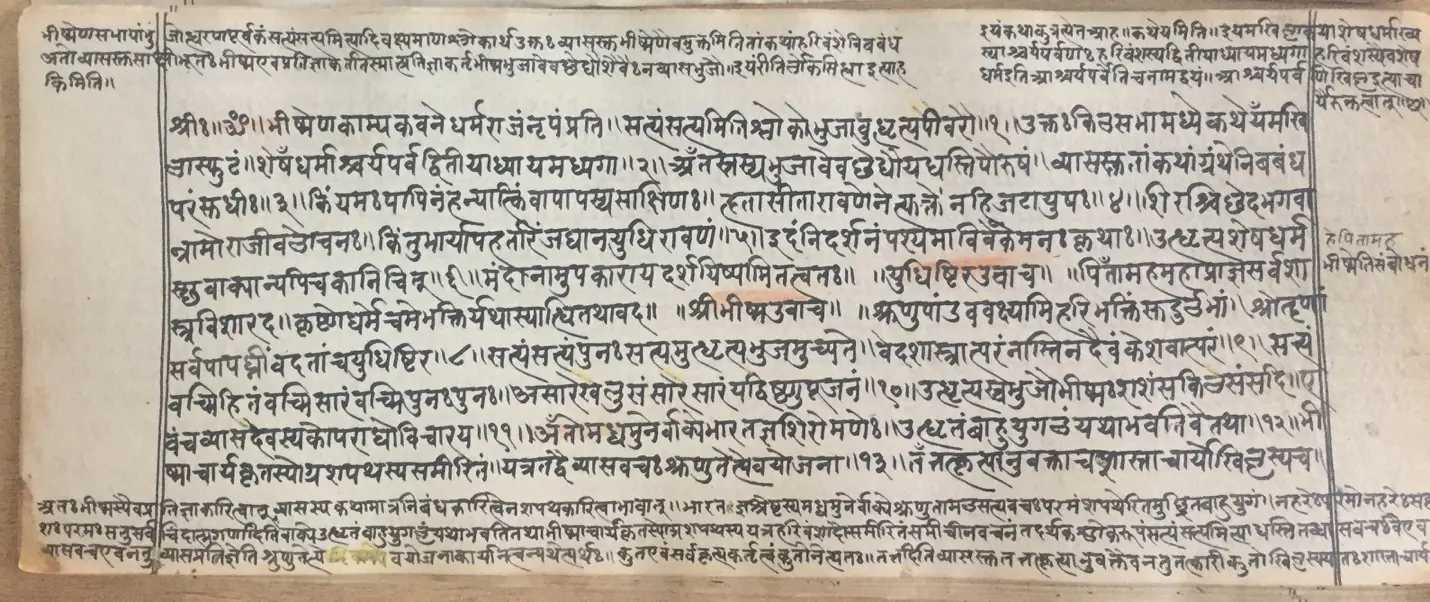
\includegraphics[width=\textwidth]{images/figure-01.jpg}
\caption{Leaf from the \emph{{Pāṣaṇḍakhaṇḍanavyāsastōtra}} with marginal commentary by an unknown author. Mysore Oriental Research Institute, ms. 4347C.}

\end{figure}


\emph{Praising Vyāsa} consists of thirty-one verses in \emph{śloka} meter. It has been published at least twice. There are no known commentaries, but a manuscript in Mysore has extensive marginal notes that function as a kind of commentary.\footnote{%
The marginalia are anonymous, but they appear to have been copied by the same scribe who copied the main text. It is not impossible that the marginal notes belong to Surōttama, who many believe to be Vādirāja’s brother. Surōttama commented on several of Vādirāja’s writings, including the \emph{{Pāṣaṇḍakhaṇḍanavyāsastōtra}}’s companion text, the \emph{{Pāṣaṇḍakhaṇḍana}}.
}
 Both the printed text and the Mysore manuscript end with a short colophon: “Vādirāja Yati has composed this praise poem to Vyāsa (\emph{vyāsastōtra}) in the form of a critique of the apostates.”\footnote{%
Vādirāja’s \emph{{Pāṣaṇḍakhaṇḍanavyāsastōtra}} (\hyperref[VP]{Rāmācārya 1911}): \emph{iti śrīvādirājayatikr̥taṁ pāṣaṇḍakhaṇḍanaṁ vyāsastōtraṁ}.
}
 Vādirāja may have called the essay a \emph{vyāsastōtra}. Or perhaps a later copyist or cataloguer supplied the title. In either case, it is worth thinking about what, exactly, makes \emph{Praising Vyāsa} a \emph{stōtra}. 


Some have suggested that \emph{stōtra}s are stylistically distinct. Yigal Bronner, for instance, understands \emph{stōtra}s as “relatively short works in verse, whose stanzas directly and repeatedly address a divinity in the vocative case.”\footnote{%
\hyperref[Bronner2007]{Bronner} (\hyperref[Bronner2007]{2007}).
}
 Others have suggested that a \emph{stōtra}’s profusion of vocatives are the linguistic outgrowth of far more profound orientation toward a subject of praise. Hamsa Stainton, for instance, suggests that \emph{stōtra}s possess a certain “vectorial” or directional quality that foregrounds the act of praise itself.\footnote{%
\hyperref[Stainton2019]{Stainton} (\hyperref[Stainton2019]{2019}).
}
 Yet \emph{Praising Vyāsa} requires that we tweak either definition. Vādirāja’s addressees are not gods or divinities, but “idiots” and “scoundrels.” Insults replace sweet vocatives. And the very title of the essay betrays a multi-vectoral devotionality in which opprobrium is not inimical to the act of supplication but is in fact vital to it.


The text has a simple structure. The first third argues against \emph{Vyāsantōḷ} on the basis of narrative-criticism. Vādirāja argues that Vyāsa is a victim of wrongful punishment. As a reporter of epic events, the thinking goes, Vyāsa was simply conveying a statement Bhīṣma had made about Viṣṇu being the ultimate lord instead of Śiva. Vīraśaivas have mutilated the messenger. The second third of the text poses a set of hypotheticals about wrongful punishment, which is followed by an argument about the \emph{liṅga} being a symbol of Śiva’s dismemberment. The first two sections give way to a description of the painted image of Vyāsa and a set of concluding verses that say any Śaiva who wants to cut Vyāsa’s arm ends up harming Śiva instead.


Vādirāja begins by describing a declaration Bhīṣma made in front of an assembly of learned men:

\begin{pullquote}\raggedright
      \emph{bhīṣmēṇa kāmyakavanē dharmarāja(ṁ) nr̥paṁ prati}\\
\emph{satyaṁ satyam iti ślōkō bhujāv uddhr̥tya pīvarau}

\emph{uktaḥ kila sabhāmadhyē kathēyam akhilā sphuṭā}\\
\emph{śēṣadharmāścaryaparvadvitīyādhyāyamadhyagā}

\emph{atas tasya bhujāv ēva chēdyau yady asti pauruṣaṁ}\\
\emph{vyāsas tu tāṁ kathāṁ granthē nibabandha paraṁ sudhīḥ}

\emph{kiṁ yamaḥ pāpinaṁ hanyāt kiṁ vā pāpasya sākṣiṇaḥ}\\
\emph{hr̥tā sītā rāvaṇēnēty uktē nahi jaṭāyuṣaḥ}

\emph{śiraś cicchēda bhagavān rāmō rājīvalōcanaḥ}\\
\emph{kiṁ tu bhāryāpahartāraṁ jaghāna yudhi rāvaṇaṁ}

\emph{idaṁ nidarśanaṁ paśya māvivekē manaḥ kr̥thāḥ}\\
\emph{uddhr̥tya śēṣadharmasthavākyāny api ca kānicit}

\emph{mandānām upakārāya darśayiṣyāmi tattvataḥ}
\end{pullquote}
      
\begin{pullquote}
Among the assemblymen in the Kāmyaka forest, Bhīṣma proclaimed the verse “this is the truth, this is the truth” to king Dharmarāja (Yudhiṣṭhira), brawny arms lifted high. This well-known tale is found in the second chapter of the Āścaryaparvan on \emph{śeṣadharma}. Therefore, the heroic thing to do would have been to cut off Bhīṣma’s arm. Vyāsa, who is exceedingly learned, simply recorded that event in the \emph{Mahābhārata}. Should Yama, the god of death, kill the sinner? Or should he kill the one who witnessed the sin? The lotus-eyed Rāma didn’t cut off Jaṭāyus’s head after he reported that Rāvaṇa abducted Sītā Rather, Rāma killed the kidnapper of his wife, Rāvaṇa, in battle. Take a look at the evidence! Don’t fix your mind on this stupidity. After quoting a few statements from the \emph{śeṣadharma} section of the \emph{Mahābhārata} to help the idiots, I will make you understand the verses as they really are.


\medskip\hfill\begin{minipage}{0.9\textwidth}\small\hfill
Vādirāja, \emph{{Pāṣaṇḍakhaṇḍanavyāsastōtra}} (\hyperref[VP]{Rāmācārya 1911}, vv. 1–7a)\end{minipage}\hspace{2em}
\end{pullquote}

Vādirāja poses a peculiar genealogy of \emph{Vyāsantōḷ}. By his account, cutting off Vyāsa’s arm is born from a misreading of the \emph{{Harivaṁśa}} (the Āścaryaparvan of the \emph{Mahābhārata}). Yet the verses he cites are not found in the Bhandarkar edition of the text or in its critical apparatus, and only one can be found in Madhva’s commentary on the \emph{Mahābhārata}, which Vādirāja invokes approvingly in the next passage. According to Vādirāja, it was Bhīṣma who lifted his arm and declared, “this is the truth, this is the truth, again, this is the truth.” Vādirāja continues:

\begin{pullquote}\raggedright
      

	\emph{yudhiṣṭhiraḥ  \Dash }\\
\emph{pitāmaha mahāprajña sarvaśāstraviśārada}\\
\emph{kr̥ṣṇē dharmē ca mē bhaktir yathā syād dhi tathā vada}



	\emph{bhīṣmaḥ  \Dash }\\
\emph{śr̥ṇu pāṇḍava vakṣyāmi haribhaktiṁ sudurlabhāṁ}\\
\emph{śrōtṝṇām sarvapāpāghnīṁ vadatāṁ ca yudhiṣṭhira}

\emph{satyaṁ satyaṁ punaḥ satyam uddhr̥tya bhujam ucyatē}\\
\emph{vēdaśāstrāt paraṁ nāsti na daivaṁ kēśavāt paraṁ}

\emph{satyaṁ vacmi hitaṁ vacmi sāraṁ vacmi punaḥ punaḥ}\\
\emph{asārē khalu saṁsārē sāraṁ yad viṣṇupūjanaṁ}

\emph{uddhr̥tya svabhujau bhīṣmaḥ śaśaṁsa kila saṁsadi}\\
\emph{ēvaṁ cēd vyāsadēvasya kō ’parādhō vicāraya}

\emph{atō madhvamunēr vākyē bhāratajñaśikhāmaṇēḥ}\\
\emph{uddhr̥taṁ bāhuyugulaṁ yathā bhavati vai tathā}

\emph{bhīṣmācāryakr̥tasyōgraśapathasyānuvāditaṁ}\\
\emph{yatra tad vai vyāsavacaḥ śr̥ṇu cēt tava yōjanā}

\emph{tattatkr̥tyānuvaktā ca śāstrācāryō ’khilasya ca}\\
\emph{aśēṣanigamōddhartā hartā duḥsamayasya ca}

\emph{manaḥsaṁkalpamātrēṇa kurupāṇḍavasēnayōḥ}\\
\emph{kartā satyavatīputrō vihartā munimaṇḍalē}

\emph{rājasūyasya cārcāyaḥ sarpayāgasya ca prabhuḥ}\\
\emph{kas tasya bhujayōś chēttā kiṁ vā tac chēdakāraṇam}

\emph{bhramamūlā tataḥ sarvā kathāsīd vyāsavairiṇām}\\
\emph{rajakadrōhatō bhikṣōḥ śūlārōpaṇavākyavat}

\emph{bhrāmakaṁ tasya śāstraṁ ca yatrētthaṁ samudīritam}
\end{pullquote}
      
\begin{pullquote}
Yudhiṣṭhira said: “O grandfather, great intellect, expert in all the sciences, teach me in such a way that I should be devoted to Kr̥ṣṇa and \emph{dharma}.” \medskip


Bhīṣma replied: “Listen up, Yudhiṣṭhira. I’ll tell you about devotion to Viṣṇu, which is very difficult to get in this world, a devotion that destroys the sins of both listeners and speakers alike. This is the truth! This is the truth! Again, this is the truth! I proclaim this lifting my arm. There is no scripture superior to the Vedas. There is no god superior to Viṣṇu. I am telling you the truth. I am describing what is beneficial for you. I am telling you again and again the essence of everything. The one essential thing in this essence-less existence is worshiping Viṣṇu.”\medskip


Lifting his arms in the air, Bhīṣma proclaimed this in the assembly of kings. If this is the way it was, why fault Vyāsa? Think about it! This is why Madhva  \Dash  the crest-jewel among those who know the \emph{Mahābhārata}  \Dash  wrote in his commentary on the \emph{Mahābhārata} that just as Bhīṣma said this while raising his arms, Vyāsa recounted it in the same way (i.e., arms raised). If only you would pay attention to Vyāsa’s speech, then your sense of the passage would be that it is a retelling of the great vow taken by Bhīṣma. Vyāsa is the narrator of this or that person’s deeds in the epic and is the teacher of the whole \emph{Mahābhārata}. He is the rescuer of the Vedas and destroyer of incorrect codes of conduct. By simply setting his mind to it, Vyāsa  \Dash  the son of Satyavatī and who relishes being in the assembly of sages  \Dash  creates the Kurus and Pāṇḍavas (in the minds of the reader) and presides over the Rājasūya, Arcā, and Sarpayāga rites. Who could cut off Vyāsa’s arms, and what is the purpose of doing so? Thus, the whole story about severing Vyāsa’s hand is, at its root, erroneous and belongs to those who hate him. This is like calling for a sage to be impaled on a spike for the crimes of a washman. And where a text prescribes cutting off Vyāsa’s arm, it does so to deceive whoever reads it.


\medskip\hfill\begin{minipage}{0.9\textwidth}\small\hfill
\hyperref[VP]{\emph{ibid.}}, vv. 7b–19.\end{minipage}\hspace{2em}
\end{pullquote}

After arguing that Vyāsa was simply relaying Bhīṣma’s sermon when he repeated the phrase, “this is the truth,” Vādirāja turns his attention to Śiva. If any god has been dismembered, Vādirāja claims, it is Śiva not Vyāsa. He cites a story from the \emph{{Padma Purāṇa}} in which Śiva, who had been distracted while having sex with Pārvatī, snubs Bhr̥gu who then chops Śiva to pieces out of anger. All that remains is Śiva’s penis mid-coitus, which is symbolized by the \emph{liṅga} that Vīraśaivas wear and worship. He writes: 

\begin{pullquote}\raggedright
      \emph{nārīsaṁgamamattō ’sau yasmān mām avamanyatē}\\
\emph{yōniliṅgasvarūpaṁ hi tasmād asya bhaviṣyati}

\emph{iti padmapurāṇōktaṁ bhr̥guśāpasya sāhasaṁ}\\
\emph{paśyantu pañcaśīrṣāṇi bhujānām ca catuṣṭayaṁ}

\emph{dvau pādāv adaraṁ vakṣaḥ kaṭī cōrū ca dhūrjaṭēḥ}\\
\emph{vichidya tatkṣaṇād ēva petuḥ kila mahītalē}

\emph{śiśnamātraṁ tūrvaritaṁ tac ca yōnyām nivēśitaṁ}\\
\emph{atra pramāṇaṁ śaivānāṁ kaṇṭhē kaṇṭhē vilaṁbinī}

\emph{liṅgamālaiva yā nityaṁ karē vāmē prapūjyatē}\\
\emph{ataḥ pādmōditakathā śaivānām api saṁmatā}
\end{pullquote}
      
\begin{pullquote}
In the \emph{{Padma Purāṇa}}, the punishment of the curse of Bhr̥gu is relayed in the following way: 
	    \medskip


“Śiva, who was out of his mind because he was having sex with his wife, disrespected me (Bhr̥gu). Because of this, Śiva’s body will be reduced to his penis in Pārvatī’s vagina. Let everyone see that after Śiva’s five heads, his four arms, his two feet, stomach, chest, hips, and thighs are chopped off, they fall to the ground in an instant. Only his penis, which had entered the vagina, remained.” \medskip


The proof for this is that around Śaivas’ throats dangle a necklace of Śiva’s penis, which they worship with the left hand. Thus, the Śaivas, too, agree with me on this story from the \emph{{Padma Purāṇa}}.


\medskip\hfill\begin{minipage}{0.9\textwidth}\small\hfill
\hyperref[VP]{\emph{ibid.}}, vv. 20–24.\end{minipage}\hspace{2em}
\end{pullquote}

The salacious provocation gives way to reverential praise, where Vādirāja invokes the “knowledge-giving image of Vyāsa” as painted on walls by artists and described in \emph{mantra} texts: 

\begin{pullquote}\raggedright
      \emph{hastadvayavatī ramyajaṭāmaṇḍalamaṇḍitā}\\
\emph{padmapādā śyāmavarṇā lasatkr̥ṣṇājinōjjvalā}

\emph{mandasmitā candramukhī bimbōṣṭhī paṅkajēkṣaṇā}\\
\emph{kundakuḍmaladantābhā sāndrakuntalasaṅkulā}

\emph{kandarpakōṭisadr̥śī saundaryāṁbudhimandirā}\\
\emph{vandārūṇām abhayadā vandyamānāsurair naraiḥ}

\emph{adyāpi pūjyatē vyāsapratimā jñānadāyinī}\\
\emph{citrakair likhyate bhittau mantraśāstreṣu varṇyate}
\end{pullquote}
      
\begin{pullquote}
Even today, the knowledge-giving image of Vyāsa is painted on walls by artists and is described in various \emph{mantra} texts  \Dash  


	
	      the image, which shows Vyāsa as having two hands;\\
	      as being lustrous with beautiful hair;\\
	      as having dark, lotus-like feet;\\
	      as luminous from the radiant antelope skin he sits on;\\
	      as smiling with happiness;\\
	      as having a moon-like face with lips like the bimba fruit;\\
	      as having lotus-like eyes and teeth like budding jasmine flowers;\\
	      as having thick hair;\\
	      the image of Vyāsa is like a crore of gods of love;\\
	      is the object of devotion for those who worship beauty;\\
	      it gives fearlessness to all those who prostrate;\\
	      and it is worshiped by both gods and humans alike.
	    \\


\medskip\hfill\begin{minipage}{0.9\textwidth}\small\hfill
Vādirāja, \emph{{Pāṣaṇḍakhaṇḍanavyāsastōtra}} (\hyperref[VP]{Rāmācārya 1911}, vv. 25–28)\end{minipage}\hspace{2em}
\end{pullquote}

Vādirāja concludes by writing: 

\begin{pullquote}\raggedright
      \emph{atō vyāsabhujacchēdam āśāsānasya durmatēḥ}\\
\emph{svadairvasarvagātrāṇāṁ chēdaḥ khēdakarō ’bhavat}

\emph{tadvr̥ddhim icchatō mūlachēdō ’bhūt tava durjana}\\
\emph{yadvyāsāya druhyatas te śivadrōhō ’bhavad dhruvaḥ}

\emph{vivādaparihārāya kathēyaṁ grathitā kila}\\
\emph{yatinā vādirājēna vyāsakaiṅkaryakāminā}

	\emph{iti śrīvādirājayatikr̥taṁ pāṣaṇḍakhaṇḍanaṁ vyāsastōtraṁ}\\

\end{pullquote}
      
\begin{pullquote}
It follows, then, that the idiot who is longing to amputate Vyāsa’s arm is tormented instead by cutting off all of your own god’s limbs. Hey, loser! You wanted interest on your capital, but you ended up losing your capital instead. By violating Vyāsa, you ended up slandering Śiva. Desiring servitude to Vyāsa, I have composed this story to solve the controversy of his arm.


\medskip\hfill\begin{minipage}{0.9\textwidth}\small\hfill
Vādirāja, \emph{{Pāṣaṇḍakhaṇḍanavyāsastōtra}} (\hyperref[VP]{Rāmācārya 1911}, vv. 29–31)\end{minipage}\hspace{2em}
\end{pullquote}

Unlike other Vyāsa \emph{stōtra}s, \emph{Praising Vyāsa} combines perfunctory textual arguments with declarations about Vyāsa’s painted image not to construct a new image of Vyāsa in the minds of readers, but to restore an image under threat. The textual and visual arguments about Vyāsa’s body amount to two intersecting axes for managing the volatility of Vyāsa’s representation. The close connection between image and text suggests that the problem of cutting Vyāsa’s arm was not simply an act of iconoclasm, but also a form of textoclasm in which the \emph{Mahābhārata} and its interpretive methods were wounded alongside Vyāsa’s body. 

\section{Piety and Paralysis at Śiva’s Doorstep}
      I want to begin a provisional genealogy of \emph{Vyāsantōḷ} by looking at an episode in the \emph{{Skanda Purāṇa}}, in which Vyāsa, who is depicted as a zealous devotee of Viṣṇu, was paralyzed and convinced of Śiva’s supremacy. That Vyāsa was the target of a type of forced conversion is unsurprising. Peter Bisschop has recently argued that the \emph{{Skanda Purāṇa}} emerged in part as a Śaiva rejoinder to the Vaiṣṇavization of the \emph{Mahābhārata}, and so any reappropriation of the epic would inevitably involve Vyāsa.\footnote{%
In Bisschop’s words, the \emph{{Skanda Purāṇa}} is where Vyāsa became “a dedicated Pāśupata adept” (\hyperref[Bisschop2021]{Bisschop 2021}: 49).
}
 In an episode in the \emph{{Kāśīkhaṇḍa}}, Vyāsa is depicted as a haughty Vaiṣṇava who wandered around haranguing sages about the glories of Hari. Once in the Naimiṣa Forest, Vyāsa found himself standing before thousands of ash-smeared Śaivas. He lifted a finger and indulged in a sanctimonious sermon: 

\begin{pullquote}\raggedright
      \emph{parinirmathya vāgjālaṁ suniścityāsakr̥d bahu}\\
\emph{idam ēkaṁ parijñātaṁ sēvyaḥ sarvēśvarō hariḥ}

\emph{vēdē rāmāyaṇē caiva purāṇēṣu ca bhāratē}\\
\emph{ādimadhyāvasānēṣu harir ēkō ’tra nāparaḥ}

\emph{satyaṁ satyaṁ trisatyaṁ punaḥ satyaṁ na mr̥ṣā punaḥ}\\
\emph{na vēdād aparaṁ śāstraṁ na dēvō ’cyutataḥ paraḥ}

\emph{lakṣmīśaḥ sarvadō ’nānyo lakṣṁīśō ’py apavargadaḥ}\\
\emph{ēka ēva hi lakṣṁīśas tatō ’dhyēyō na cāparaḥ}

\emph{bhuktēr muktēr ihānyatra nānyō dātā janārdanāt}\\
\emph{tasmāc caturbhujō nityaṁ sēvanīyaḥ sukhēpsubhiḥ}

\emph{vihāya kēśavād anyaṁ yē sēvantē ’lpamēdhasaḥ}\\
\emph{saṁsāracakrē gahane tē viśanti punaḥ punaḥ}

\emph{ēka ēva hi sarvēśō hr̥ṣīkēśaḥ parāt paraḥ}\\
\emph{taṁ sēvamānaḥ satataṁ sēvyas trijagatāṁ bhavēt}

\emph{ēkō dharmapradō viṣṇus tv ēkō bahvarthadō hariḥ}\\
\emph{ēkaḥ kāmapradaś cakrī tv ēkō mōkṣapradō ’cyutaḥ}

\emph{śārṅgiṇaṁ yē parityajya dēvam anyam upāsatē}\\
\emph{tē sadbhiś ca bahiṣkāryā vēdahīnā yathā dvijāḥ}
\end{pullquote}
      
\begin{pullquote}
After churning a vast ocean of words, and after becoming perfectly sure of their meaning time and again, I’ve come to know this one thing  \Dash  Hari is the one who should be worshiped. Hari is the lord of all. From beginning to end, the Vedas, \emph{Rāmāyaṇa}, Purāṇas, and \emph{Mahābhārata} convey only Hari and no one else. This is the truth! This is the truth! Again, this is the truth! A triple oath. It’s not wrong to say that there is no scripture greater than the Vedas, no god greater than Hari. No one but the Lord of Lakṣmī is the giver of all, and no one but Lakṣmī is the giver of heaven. Because the Lord of Lakṣmī is the one and only, it follows that he should be worshiped and no one else. No one but Janārdana gives enjoyment in this world and liberation hereafter. Thus, those who want happiness should always serve Viṣṇu. Having abandoned him, the stupid people who worship another god consign themselves again and again to the mysterious cycle of \emph{saṁsāra}. Indeed, there is only one lord of all. Hr̥ṣīkēśa is the best of the best. Whoever attends to him would themselves be the object of constant worship of the three worlds. Only Viṣṇu is the giver of \emph{dharma}. Only Hari is the giver of riches. Only the Discus-Bearer is the giver of pleasure. And only Acyuta is the giver of liberation. Those who forsake the Archer and worship another god should be abandoned by the virtuous, like a Dvija who has lost the Vedas.


\medskip\hfill\begin{minipage}{0.9\textwidth}\small\hfill
\emph{{Skāṇḍapurāṇīyakāśīkhaṇḍa}} (\hyperref[Kasikhanda1908]{Śrēṣṭhin 1908}, vv. 95.11–19, fol. 351v)\end{minipage}\hspace{2em}
\end{pullquote}

The Śaiva sages of the Naimiṣa Forest revered Vyāsa for arranging the Vedas and authoring the \emph{Mahābhārata}, but his homily made them agitated. The sages spoke up: “The people here don’t trust what you have just argued with your finger raised confidently. But we would trust you if you proclaim it in front of Śiva in Benares.”\footnote{%
\emph{{Skāṇḍapurāṇīyakāśīkhaṇḍa}} (\hyperref[Kasikhanda1908]{Śrēṣṭhin 1908}, vv. 95.23–25, foll. 351v–352r):

\vspace{-1.5ex}\begin{quote}\raggedright
      \emph{bhavatā yat pratijñātaṁ niścityōtkṣipya tarjanīm}\\
\emph{asmin māṇavakās tatra pariśraddadhatē na hi}\\
\emph{pratijñātasya vacasas tava śraddhā bhavēt tadā}

\emph{yadānandavanē śaṁbhōḥ pratijānāsi vai vacaḥ}\end{quote}\vspace{-1.5ex}
      }
 Annoyed, Vyāsa set off for Śiva’s city with his entourage. Their time in Benares began wondrously: Vyāsa bathed at the city’s ghats and performed rites for Viṣṇu. Conch-calls announced his presence. Devotees adorned him with fresh garlands of Tulasi. And he sang the lord’s many names in the streets. It was in the buoyant din of devotion that Vyāsa and his followers danced their way to Śiva’s doorstep at the Viśveśa Temple. They sang some more, and when the music stopped, Vyāsa stood there among his students. “He lifted his right arm,” the passage reads, “and he loudly recited the Naimiṣa sermon again, this time as if it were song  \Dash  ‘After churning a vast ocean of words, and after becoming perfectly sure of their meaning time and again, I’ve come to know this one thing  \Dash  Hari is the one who should be worshiped, Hari is the lord of all.’”\footnote{%
\emph{{Skāṇḍapurāṇīyakāśīkhaṇḍa}} (\hyperref[Kasikhanda1908]{Śrēṣṭhin 1908} v. 95.44, fol. 352r):

\vspace{-1.5ex}\begin{quote}\raggedright
      \emph{punar ūrdhvaṁ bhujaṁ kr̥tvā dakṣiṇaṁ śiṣyamadhyagaḥ}\\
\emph{punaḥ papāṭha tān ēva ślōkān gāyann ivōccakaiḥ}

\emph{parinirmathya vāgjalāṁ suniścityāsakr̥d bahu}\\
\emph{idam ēkaṁ parijñātaṁ sēvyaḥ sarvēśvarō hariḥ}\end{quote}\vspace{-1.5ex}
      }


\begin{figure}[ht!]\label{fig2}\centering

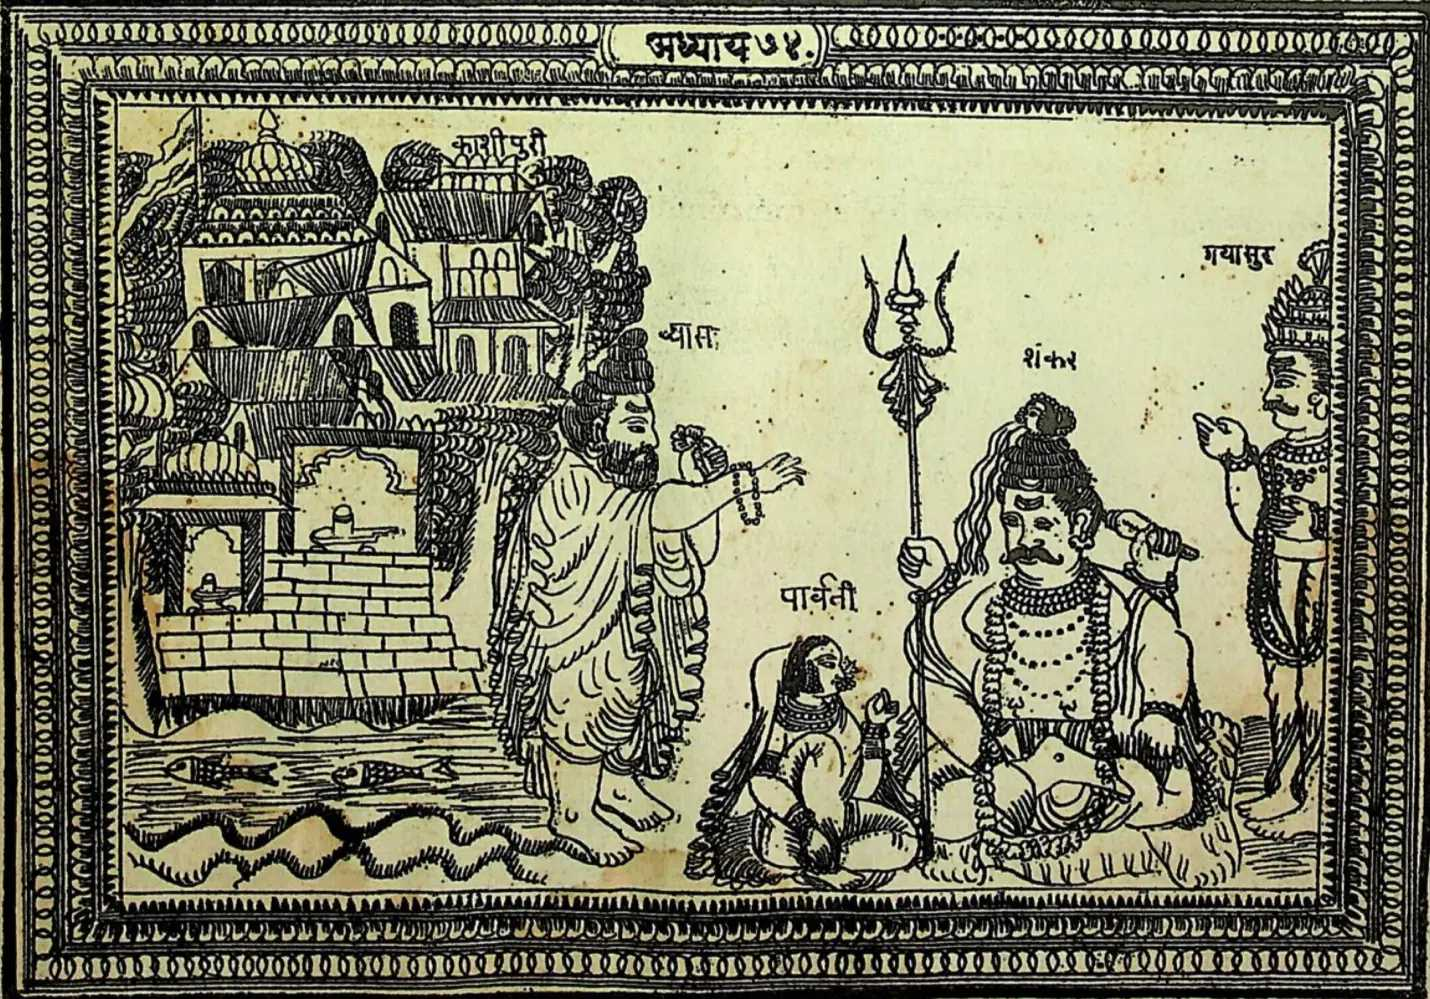
\includegraphics[width=\textwidth]{images/figure-02.jpg}
\caption{Lithograph of Vyāsa lifting his right arm while proclaiming to Śiva that Viṣṇu is the supreme lord. Frontispiece of the 74th chapter of a Marathi translation of the Kāśīkhaṇḍa (1881).}

\end{figure}


Vyāsa the pious provocateur became a chapter frontispiece for a Marathi translation of the \emph{{Kāśīkhaṇḍa}} published in 1881. The lithograph shows Vyāsa standing in front of Śiva and Pārvatī, right arm lifted as he pronounces Viṣṇu the lord of all. In the Marathi edition, Gayāsura is the one who points his finger and curses Vyāsa. The more popular telling has Śiva’s attendee Nandin doing the cursing. In both, Vyāsa’s arm became stiff and his voice faltered mid-sermon. For all the dancing and singing, Vyāsa could never quite summon Viṣṇu. But in the silent paralysis of Nandin’s curse, Viṣṇu finally appeared. Rather than praise Vyāsa for his devotion, however, Viṣṇu admonished him. “O Vyāsa! You’ve committed a serious sin. Even I’m terrified by your offense.”\footnote{%
\emph{{Skāṇḍapurāṇīyakāśīkhaṇḍa}} (1908), vss. 95.48b–49a, fol. 352v:

\vspace{-1.5ex}\begin{quote}\raggedright
      \emph{aparādhaṁ mahac cātra bhavatā vyāsa niścitam}\\
\emph{tavaitad aparādhēna bhītir mē ’pi mahattarā}\end{quote}\vspace{-1.5ex}
      }
 Viṣṇu explains: 

\begin{pullquote}\raggedright
      \emph{ēka ēva hi viśvēśō dvitīyō nāsti kaścana}\\
\emph{tatprasādād ahaṁ cakrī lakṣmīśas tatprabhāvataḥ}\\
\emph{trailōkyarakṣāsāmārthyaṁ dattaṁ tēnaiva śambhunā}\\
\emph{tadbhaktyā paramaiśvaryaṁ mayā labdhaṁ varāt tataḥ}\\
\emph{idānīm stuhi śaṁbhuṁ yadi mē śubham icchasi}
\end{pullquote}
      
\begin{pullquote}
Śiva is the one true lord of the universe. There’s no second. His grace makes me the discus bearer, his power makes me Lakṣmī’s husband. It’s Śambhu who gives me the ability to protect the three worlds. It’s only by devotion to Śiva that he granted me divine status as a boon. If you desire my welfare, praise Śambhu.


\medskip\hfill\begin{minipage}{0.9\textwidth}\small\hfill
\emph{{Skāṇḍapurāṇīyakāśīkhaṇḍa}} (\hyperref[Kasikhanda1908]{Śrēṣṭhin 1908}, vv. 95.49b–51, fol. 352v)\end{minipage}\hspace{2em}
\end{pullquote}

Still speechless, Vyāsa gestured for Viṣṇu to restore his speech. Viṣṇu obliged, and Vyāsa (arm still paralyzed) praised Śiva as the ultimate lord with eight verses (a \emph{{Vyāsāṣṭaka}} of a different kind).


Paralysis was only the beginning of Vyāsa’s difficulties in Kāśī. Hunger, desperation, and, in some tellings, exile would await him after Nandin lifted the curse.\footnote{%
Skanda goes on to narrate the famous episode of Vyāsa’s hunger in Kāśī. The fourteenth-century Vīraśaiva and Telugu poet Śrīkaṇṭha used this episode in his \emph{{Bhīmēśvarakhaṇḍamu}} to foreground Vyāsa’s exile from Kāśī and his arrival at Dakṣarāma. See \hyperref[Rao2012]{Narayana Rao and Shulman} (\hyperref[Rao2012]{2012}: 76–81).
}
 Yet of all Vyāsa’s travails, his paralyzed arm proved an especially potent subject of poetic focus. The Telugu poet Śrīnātha elaborated on this episode in his \emph{{Kāśīkhaṇḍamu}}, and it appears to have migrated out of the Purāṇas altogether and circulated as a standalone work.\footnote{%
Śrīnātha, \emph{{Kāśīkhaṇḍamu}} 7.103–110 in \hyperref[Rao1990]{Narayana Rao and Roghair} (\hyperref[Rao1990]{1990}: 281, n. 29).
}
 For instance, a short manuscript at the Rajasthan Oriental Research Institute in Jodhpur titled \emph{Praising the Paralysis of Vyāsa’s Arm} (\emph{{Vyāsabhujastambhanastōtra}}) recounts Vyāsa’s paralysis in Kāśī in the form of praise poem.\footnote{%
\emph{{Vyāsabhujastambhastōtra}} (1984), p. 266.
}


\begin{figure}[ht!]\label{fig3}\centering

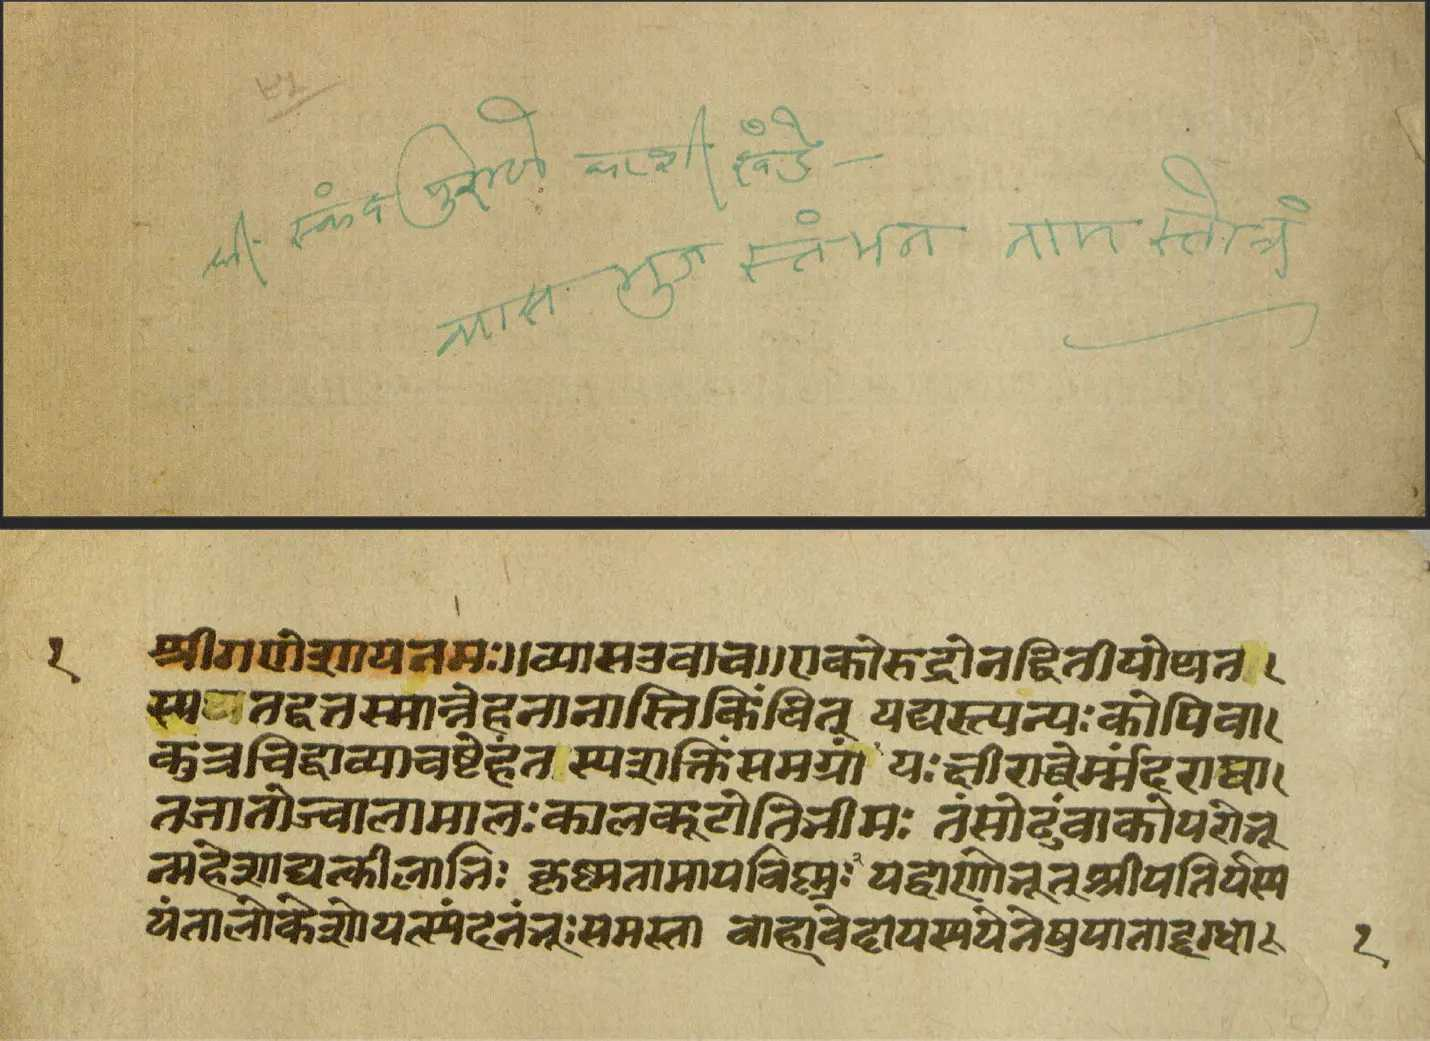
\includegraphics[width=\textwidth]{images/figure-03.jpg}
\caption{Leaf from the \emph{{Vyāsabhujastambhanastōtra}}. Rajasthan Oriental Research Institute, ms. no. 2392. The inscription in green ink reads \emph{śrīskandapurāṇē kāśīkhaṇḍē vyāsabhujastaṁbhana(ṁ) nāma stōtram}.}

\end{figure}


In both the \emph{{Skanda Purāṇa}} and \emph{Praising Vyāsa}, Vyāsa lifts his arm and proclaims his triple oath about Viṣṇu’s supremacy  \Dash  “This is the truth! This is the truth! Again, this is the truth!” In the \emph{{Skanda Purāṇa}}, Vyāsa’s declaration is his own, whereas in \emph{Praising Vyāsa} it is Bhīṣma’s. Vādirāja does not mention what happens to Vyāsa’s voice, but the \emph{{Skanda Purāṇa}} positions aphonia alongside monoplegia as connected afflictions. Vyāsa’s arm is simply an extension of a pious speech act, and its uplifted position a gesture of steadfast devotion. It is the arm’s connection to Vyāsa’s Viṣṇu worship that transformed it into a location for, and an eventual symbol of, the rejection of the belief of Viṣṇu's supremacy over Śiva.


The arm as a site of divine intervention is a well-worn trope. Vyāsa’s paralysis in Kāśī mirrors an episode in the Drōṇaparvan of the \emph{Mahābhārata}, where the infant Śiva paralyzed Indra’s uplifted arm just as Indra was about to kill him with a lightning bolt.\footnote{%
\emph{Mahābhārata}, \emph{Drōṇaparvan}, v. 7.173.60.
}
 The \emph{{Śivadharmōttara}} (ca. seventh century \textsc{ce}), for instance, describes a variety of divine afflictions: the Sun has leprosy, Varuṇa has dropsy, Pūṣan is missing teeth, Soma has consumption, Dakṣa Prajāpati has a fever, and Indra has a paralyzed arm (\emph{bhujastambha}). The \emph{{Śivadharmōttara}} and the later Tamil \emph{{Civatarumōttaram}} (ca. sixteenth century \textsc{ce}) do not specify Śiva’s role in Indra’s paralysis, but the \emph{{Taṇikaipurāṇam}} (ca. eighteenth century \textsc{ce}) clarifies that it was indeed Śiva who brought on these afflictions.\footnote{%
See \emph{{Śivadharmōttara}} (\hyperref[Sivadharmottara]{2019}), vv. 8.224-25. Thanks are due to Jesse Pruitt for bringing these verses to my attention.
}



The paralysis of Indra’s arm in the \emph{Mahābhārata} and \emph{{Śivadharmōttara}} may have provided a template for the story of Vyāsa’s paralysis in Kāśī. Amputation is medically distinct from paralysis, but their narrative forms are distinguished only by degrees of permanence. The severing of Vyāsa’s arm is different from the paralysis of Vyāsa’s arm because it is a permanent intervention in a pious gesture instead of a temporary one. Amputation is perhaps best understood as an inevitable amplification of the kind of bodily interventions Śiva had long been depicted as exercising over other gods. The drift from paralysis to amputation is difficult to track, but it is evident in faint traces in Vīraśaiva writings from the sixteenth and seventeenth centuries, where Purāṇic accounts of Vyāsa’s paralysis became a reference point for prescribed interventions against Śiva’s naysayers and critics.


The ninth chapter of the \emph{{Siddhāntaśikhāmaṇi}} of Śivayōgin (ca. mid-thirteenth century \textsc{ce}), for instance, enumerates a pious Śaiva’s ideal conduct and their salvific rewards.\footnote{%
Here I take M.\thinskip{}R. Sakhare’s dates. See \hyperref[Sakhare1942]{Sakhare} (\hyperref[Sakhare1942]{1942}: 370).
}
 Many dictates concern matters of conduct, almsgiving, and ritual purity. But a handful of others promote a punitive strategy against Śiva’s enemy’s  \Dash  “one should be ready to martyr themselves to protect a \emph{liṅga} and its devotees from destruction,” reads one verse.\footnote{%
Śivayōgin, \emph{{Siddhāntaśikhāmaṇi}} (\hyperref[Sivayogin2015]{Śivakumāra 2015}, v. 9.34–35).
}
 Another reads: 

\begin{pullquote}\raggedright
      If you see someone criticizing Śiva, then you should hurt them (\emph{ghātayēt}), or (in the least) you should curse them (\emph{śapēt}). If you can’t do either, then you should turn from that place and go away.\footnotemark{}

\end{pullquote}
      \footnotetext{Śivayōgin, \emph{{Siddhāntaśikhāmaṇi}} (\hyperref[Sivayogin2015]{Śivakumāra 2015}, v. 9.36). The causative imperative verb \emph{ghātayēt}, from the root \emph{han} in the sense of violence (\emph{hiṁsā}) or going (\emph{gati}), is perhaps intentionally underdefined.
}

For Maritōṇṭadārya, a commentator who lived between the fifteenth and eighteenth centuries, “to hurt” Śiva’s enemies was an insufficiently harsh reading of the verb \emph{ghātayēt}.\footnote{%
\emph{Tōṇṭada} in old Kannada means “garden.” Tiziana \hyperref[Ripepi1997]{Ripepi} (\hyperref[Ripepi1997]{1997}) has argued that as a name or title, Tōṇṭada only came into circulation after the Vijayanagara ruler Virūpākṣa, whose guru was given the title \emph{Tōṇṭada Siddhaleṅgēśvara}. Ripepi disagrees with Jan Gonda, who dates Maritōṇṭadārya to the fifteenth century. She suggests instead that he lived in the eighteenth century.
}
 Śiva’s enemies should be cursed or killed, and to support this, Maritōṇṭadārya classifies the verse under the heading “The Conduct of Vīrabhadra and Nandin” (\emph{vīrabhadrācāranandikēśvarācāra}).\footnote{%
In some recensions the heading reads, “The Conduct of Vīrabhadra and Basavēśvara” (\emph{vīrabhadrācārabasavēśvarācāra}), which pairs with the mandate to turn away and leave if one is not able to curse or beat, which is an homage to a story of Basava leaving Kalyāṇa after the city was overrun and looted by marauding anti-Śaivas.
}
 The reference is clear: In the eighty-ninth chapter of the \emph{{Skanda Purāṇa}}, just a few chapters before Vyāsa’s paralysis, Dakṣa hosted an enormous sacrifice but did not invite Śiva. Worried that Dakṣa’s irreverence will spread to others, Śiva commanded Vīrabhadra to destroy the sacrificial grounds. The result was a bloodbath. Vīrabhadra and his gang destroyed the sacrificial pavilion. They dug up the altars, drank the oblations, crushed the utensils, and devoured the sacrificial animals. Drunk on power, they massacred those who attempted to flee  \Dash  they castrated Vāyu and cut off Sarasvatī’s nose. Aditi lost his lips, Aryaman his arms, Agni his tongue. Viṣṇu  \Dash  the source of Dakṣa’s strength and the recipient of the sacrifice  \Dash  was nearly killed, but a voice from the heavens intervened just as Vīrabhadra was about to sink a trident into his chest. Vīrabhadra redirected his rage to Dakṣa, whom he swiftly bludgeoned to death with bare knuckles. Dakṣa’s demise was hardly the end of the butchery. Those who had not yet fled were methodically dismembered and hung from the sacrificial post.


Maritōṇṭadārya seems to have had Vīrabhadra’s murderous rage in mind when glossing the verb \emph{ghātayēt} as “the conduct of Vīrabhadra,” that is, “mutilating and murdering Śiva’s enemies.” Perhaps Maritōṇṭadārya found the end of the chapter, where Śiva, dismayed by Vīrabhadra’s savagery, brought his victims back to life, an unsatisfactory coda to apostasy, for he never recommends taking pity on those who speak ill against Śiva or his followers. Or perhaps Śiva’s mercy for those who were righteously slain was precisely what made violence palatable, even if only notionally. Regardless, Maritōṇṭadārya linked the second verbal action  \Dash  “should curse” (\emph{śapēt})  \Dash  to the story of Nandin and Vyāsa’s arm just a few chapters later, thus presenting butchery and bodily maiming as a logical concatenation of cursing.\footnote{%
For Śivayōgin, cursing and beating are complimentary responses to critics, but there’s no reason to suspect that he had the \emph{{Skanda Purāṇa}} in mind when writing the verse.
}



Like most scriptural dictates, Maritōṇṭadārya’s prescriptions mapped unevenly onto life on the ground. Critics of Vīraśaivism like Vādirāja Tīrtha  \Dash  who was historically and regionally proximate to Maritōṇṭadārya  \Dash  were, so far as we know, never cursed, beaten, or tortured for their dissenting views, despite having brushed shoulders with south India’s most powerful Vīraśaiva warlords. In fact, the opposite was true. The Vīraśaiva kings at Keḷadi and Ikkeri, erstwhile vassals of Vijayanagara who controlled what is now western Karnataka, Goa, and the Kanara coasts, lavished Vādirāja and other putative critics of Vīraśaivism, including Jains and Muslims, with royal largesse.\footnote{%
See \hyperref[Peterson2023]{my essay} (\hyperref[Peterson2023]{2023}) on Vādirāja’s \emph{{Pāṣaṇḍakhaṇḍana}}  \Dash  an anti-Jain essay  \Dash  for more on these patronage connections.
}
 Perhaps, then, cutting Vyāsa’s arm was realpolitik, a calculated displacement of a perilous, even impossible, command onto a symbolically potent figure. Why waste energy on an ordinary slanderer when Vyāsa, “the paragon of Vedic Brahmanical \emph{r̥ṣi}-hood,” to borrow Christopher Minkowski’s words, is available instead?\footnote{%
\hyperref[Minkowski1989]{Minkowski} (\hyperref[Minkowski1989]{1989}: 420).
}


\section{Conclusion: Contesting \emph{Vyāsantōḷ} in Colonial Courts}
      Vādirāja, Śivayōgin, and Maritōṇṭadārya (to say nothing of Purāṇas and epics) leave a crucial question unanswered: how was \emph{Vyāsantōḷ} practiced in the late sixteenth and early seventeenth centuries? Vādirāja argues against the practice on textual grounds. Its proponents have confused or exploited the labyrinthine dialogues and frame stories of the \emph{Mahābhārata} and pilloried Vyāsa for a declaration that was not his. By the early nineteenth century, however, when the Vīraśaivas of Kolhapur were preparing Vyāsa’s arm for display in the city’s streets, \emph{Vyāsantōḷ} had spilled well beyond the written page. What follows is hardly an exhaustive account of this transition, but I want to conclude by way of a provisional sketch of \emph{Vyāsantōḷ}’s juridical life in the nineteenth and twentieth centuries.


Vādirāja does not treat \emph{Vyāsantōḷ} as a processional practice, but epigraphic evidence suggests that Vīraśaivas may have incorporated Vyāsa’s arm into a fixed pillar or mobile pole adorned with a flag of Nandin and other decorations (aptly called the \emph{{Nandikamba}}) sometime before the nineteenth century. In the early 1870s, Colonel John Mackenzie made a sketch of a stone tablet in Mysore that depicts a man and woman at the base of a fixed pillar mounted with a large arm. The woman touches the pillar while the man next to her brandishes a scythe or sword. Mackenzie labeled the image \emph{Vyāsana tōḷu-kattu}  \Dash  “cutting off Vyāsa’s arm.” 

\begin{figure}[ht!]\label{fig4}\centering

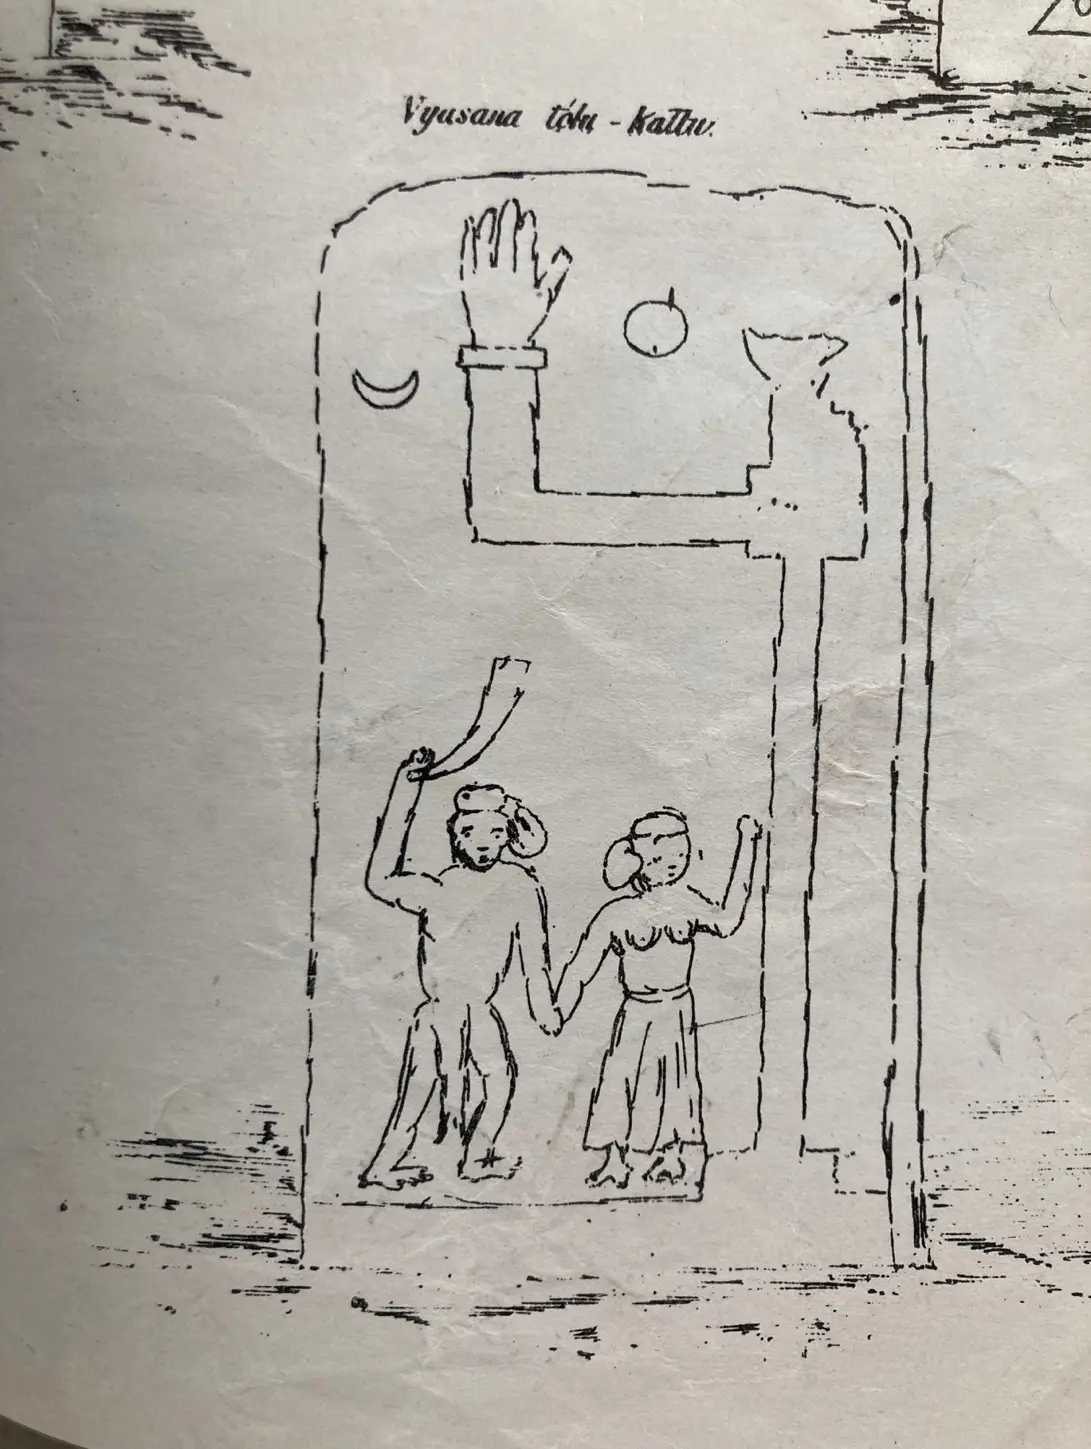
\includegraphics[width=0.8\textwidth]{images/figure-04.jpg}
\caption{Col. J.\thinskip{}S. F. Mackenzie’s sketch of a stone tablet depicting the Nandikamba, Vyāsantōḷ, and a pious Vīraśaiva couple. After much searching, I was never able to locate the tablet or an estampage. See \hyperref[Mackenzie1873]{Mackenzie} (\hyperref[Mackenzie1873]{1873}: 49).}

\end{figure}


The pillar on the tablet appears to be fixed, perhaps even made of stone, but it nevertheless resembles the kind of objects that were vigorously litigated in the nineteenth and twentieth centuries. Processional \emph{{Nandikamba}}s were made of bamboo and festooned with streamers, bells, brass globes, and, before it was outlawed, an effigy of Vyāsa’s arm and Nandin’s horn (\emph{nandikōḍu}). Even today, Vīraśaivas parade an armless \emph{{Nandikamba}} through the streets of villages and towns in northern Karnataka and southern Maharashtra.


A comprehensive study of \emph{Vyāsantōḷ}’s path through District and High Courts warrants a separate study and is beyond the scope of this article. What I present here is selective and sketchy, consisting mostly of cases presented before the Bombay High Court in the early and mid-twentieth century. A richer story will surely emerge from a close study of court archives, judge’s notes, case records, private collections, and local newspapers. But even a cursory examination of the available legal material shows how the story of \emph{Vyāsantōḷ} in colonial India is really a story about the definition of religion and its place in public life.


It is unclear precisely when, and through what legal pathways, \emph{Vyāsantōḷ} became a subject of litigation, but records attest to district-level courts in the Deccan hearing civil cases in 1881 and probably earlier.\footnote{%
See \hyperref[Oppert1893]{Oppert} (\hyperref[Oppert1893]{1893}: 58 n. 57), where Oppert mentions a decision at the Cittur Jilla court in 1881.
}
 Gazetteers and other records suggest that \emph{Vyāsantōḷ} was unevenly practiced throughout the Deccan and that no discernible consensus had emerged about its legal standing before the first decades of the twentieth century, after which a series of high-profile cases wound their way to the Bombay High Court and tested settled decisions about religious processions and more technical matters of procedure. 


In July of 1910, Lingayats in Athani, a small town in the Bijapur District of the erstwhile Bombay Presidency, petitioned the Collector of Belgaum to approve a \emph{Vyāsantōḷ} procession planned for September 20. Like the Kolhapur procession a year later, they hoped to commemorate the arrival of a prominent monastic leader. Similar events on the Kanara coast had been approved despite resistance from local Brahmans. The Vīraśaivas of Athani informed Collector B. A. Brenson of these earlier processions. After a month or so of deliberation, Brenson approved the Lingayats’ request, albeit with clear instructions for where and how the procession should take place. Brenson wrote: 

\begin{pullquote}
I therefore allow the Lingayats of Athani to hold a \emph{Vyāsantōḷ} procession after the termination of the Ganesh festival. The procession will be allowed to take place in Athani town on the 20th September 1910, between the hours of 8 and 10 AM. It will enter the town at the Siddheshwar Gate, pass through the Aditwar Peth, the road connecting the latter with the Buddhwar Peth, and then down the Buddhwar Peth to the Gachin Math, where it will terminate at 10 AM. In this quarter of the town the residents are nearly all Lingayats. The Police Sub-Inspector will conduct the procession with a sufficient force to prevent any possible disturbance.


\medskip\hfill\begin{minipage}{0.9\textwidth}\small\hfill
\hyperref[Pandurang]{\emph{Pandurang Shidrao v. Revapa Rudrapa Mohajan}} (\hyperref[Pandurang]{1910}).\end{minipage}\hspace{2em}
\end{pullquote}

Pandurang Shidrao Gumaste Patil and other “Brahmans and non-Lingayats” appealed Brenson’s decision to M. C. Gibbs, Commissioner of the Southern Division. In a fragile victory for the Lingayats, Gibb’s declared on the 15th of September  \Dash  four days before they were due to take to the streets  \Dash  that Brenson’s decision was sound and that \emph{Vyāsantōḷ} could take place. In a bid to halt the procession, Patil and the others filed an ex-parte application to the Bombay High Court. The \emph{Times of India} reported that the justices, aware of scheduled police presence and the potential for unrest, were “reluctant to grant an order at the eleventh hour on an ex-parte application.” Yet the court succumbed to the situation and halted the procession until the “matter could be decided on merits.”\footnote{%
\hyperref[ToI1910a]{\emph{Times of India}} (\hyperref[ToI1910a]{October 1910}).
}
 The Lingayats of Athani would never march.


While reporting on the case, the \emph{Times of India} explained \emph{Vyāsantōḷ} to its educated, Anglophone readership: 

\begin{pullquote}
The word “Vyasantol” literally meant the “arm of Vyas.” It was carried in procession on the top of a long pole in pursuance of a legend that Vyas, the composer of the Mahabharat epic and the other Hindu Puranic Shastras, was a great devotee of Vishnu in preference to Shiva. The arm which he had raised in devotion to Vishnu was therefore lopped off by a devotee of Shiva. In commemoration of this episode the arm was carried in public procession by the Lingayats who proposed themselves to be the ardent devotees of Shiva. The Brahman applicants on the other hand averred that this processional conveyance of the lopped limb of a sage man and sacred person like the muni Vyas, whom they held in considerable veneration was insulting, offensive, and revolting to their religious sentiments.


\medskip\hfill\begin{minipage}{0.9\textwidth}\small\hfill
\hyperref[ToI1910a]{Times of India} (\hyperref[ToI1910a]{October 1910})\end{minipage}\hspace{2em}
\end{pullquote}

Despite being “revolting” to the “religious sentiments” of some, \emph{Vyāsantōḷ} was never litigated on the basis of blasphemy law. The case before the Court concerned the right of religious procession and the authority of a District Magistrate to approve and oversee it. On  October 14, the Bombay High Court ruled against Patil and the Brahman applicants, citing earlier cases that protected religious procession in public streets, including a judgment the court had issued just months earlier about a Lingayat parade in Deshnur (a controversy involving an automobile).\footnote{%
The cases are \hyperref[Sadagopachariar]{\emph{Sadagopachariar v. A. Rama Rao}} (\hyperref[Sadagopachariar]{1902}), which was followed in \hyperref[Baslingappa]{\emph{Baslingappa Parappa Chedachal v. Dharmappa Basappa Chedachal}} (\hyperref[Baslingappa]{1910}).
}



Newspapers played an important role both in bringing \emph{Vyāsantōḷ} to a wider readership and in amplifying misinformation.\footnote{%
See for instance a piece titled “Behind the Indian Veil: Faiths and Feuds” (\hyperref[ToI1910b]{\emph{Times of India}, November 1910}). The anonymous author named “an Indian” suggests that it was Virabhadra who cut off Vyāsa’s arm.
}
 A year after the Athani court case, the \emph{Times of India} reported from so-called “vernacular sources” about a marauding band of Lingayats in Bagalkot, a small town in the Bijapur District. In addition to parading Vyāsa’s arm through the town’s streets, the \emph{Times} reported, the Lingayats “defiled” the town’s Viṭṭhala temple, carried their guru’s palanquin “cross-wise” through the streets (an honor evidently restricted to Brahmans), and “committed on the Brahman residents numerous and unprovoked assaults.” The story was not true. The \emph{Times} ran a brief press report on November 9 titled “Disturbance at Bagalkot” clarifying that Vyāsa’s arm had in fact not been paraded, that Lingayats had every right to parade their guru “cross-wise,” and that “the few individuals who did receive injuries seem to have provoked them (the Lingayats) by wantonly meddling with a lawful procession.”\footnote{%
\hyperref[ToI1911]{Times of India} (\hyperref[ToI1911]{1911}).
}



After the Bombay High Court dismissed the Athani Brahman’s ex parte application in October 1910 and sent \emph{Vyāsantōḷ} back to lower civil courts, an atmosphere of legal ambiguity seems to have provided an opening for Vīraśaivas elsewhere in the Deccan to hold their own \emph{Vyāsantōḷ} processions. Rajarshi Shahu  \Dash  the Maharaj of Kolhapur who approved the parade in May 1911 and promised his marching band to boot  \Dash  cited the Athani case as a reason for allowing the procession to proceed. But this favorable ambiguity would be short lived. On May 6, 191, just a week before the procession was due to take place in Kolhapur, Government Resolution no. 2658 was passed, which not only banned \emph{Vyāsantōḷ} in Athani, but in the District of Belgaum “for all time.”\footnote{%
\hyperref[ToI1916]{Times of India} (\hyperref[ToI1916]{1916}).
}
 The Lingayats of Athani swiftly sued. 


A lengthy appeals process in lower courts meant that the Bombay High Court would not decide another case on \emph{Vyāsantōḷ} until 1916. \hyperref[Dundappa]{\emph{Dundappa Mallappa Sigandhi and Others v. Secretary of State for India and Others}} would prove a more complex and consequential case than the ex parte application of 1910. Having done considerable research, the judges (one of whom presided over the 1910 case) wrote that \emph{Vyāsantōḷ} had been the subject of acrimonious litigation and civil conflict for more than a century and that a dispute about the right to parade Vyāsa’s arm had “always existed.”\footnote{%
\hyperref[Dundappa]{\emph{Dundappa Mallappa Sigandhi and Others v. Secretary of State for India and Others}} (\hyperref[Dundappa]{1916}).
}
 They specified that it was “Vaishnavite Brahmans” who were “most directly aggrieved,” but that Śaiva Brahmans and “non-Lingayat Hindus” sympathize with an “agitation against the procession.”\footnote{%
\hyperref[Dundappa]{\emph{Sigandhi v. Secretary of State}} (\hyperref[Dundappa]{1916}).
}



Despite \emph{Vyāsantōḷ} being an “obnoxious” and “unbecoming ceremony,” according to the defendants’ council, \emph{Vyāsantōḷ} appeared to be on firm legal footing for two reasons: First, the way in which the Government Resolution had been upheld in lower courts was illegal (the details of which need not be dealt with here).\footnote{%
It had been upheld on the basis of the District Police Act (Bom. Act IV of 1890), which, the defendants argued, allowed the Government not to “prohibit” \emph{Vyāsantōḷ} per se, but to deny future applications for its procession in perpetuity across the whole district. 
}
 Second, religious procession was a right that had been secured some years earlier by the Bombay High Court itself. The judges ruled in favor of the Lingayats once again. 


Two cases decided by the Bombay High Court secured the right to religious procession. The first, \hyperref[Sadagopachariar]{\emph{Sadagopachariar v. A. Rama Rao}} (\hyperref[Sadagopachariar]{1907}), concerned a century-long dispute between Vadakalai and Tenkalai Vaiṣṇavas over the use of streets around the Devanatha Swamy Temple in Thiruvanthipuram and its adjoining shrine dedicated to Vedānta Deśika, an important Vadakalai guru. After a century of legal wrangling, the Court ruled in 1907 that the public have a right to use city streets, even those adjoining prominent temples.\footnote{%
In 1807, Tenkalais in Thiruvanthipuram sued Vadakalais for having been prevented from installing an image of a Tenkalai guru in the Devanatha Swamy Temple. The Tenkalais lost the suit but installed the image in a nearby house and began parading it in the streets around the temple. The Vadakalais sued in response, alleging that the streets around the temple were originally the property of Vadakalais who permitted the construction of houses on the condition that no “alien deity” be worshiped in them or processed on nearby streets. The court consulted a handful of sympathetic pandits who, the 1907 judges remark, based their decision “not so much on legal grounds as on precepts relating to ritual and ceremonial observances to be found in the ancient treatises on such subjects.” The Vadakalais won their case but there were numerous suits and countersuits until 1886, when the Magistrate of the Southern Arcot District refused to prohibit the public procession of Tenkalai images. Vadakalais lost on appeal and then brought the case to the Bombay High Court. The Court determined that there was no evidence attesting to the streets surrounding the temple belonging to Vadakalais. To the contrary, the streets belonged to the public under Madras Act No. V of 1884. See \hyperref[Baslingappa]{\emph{Baslingappa Parappa Chedachal v. Dharmappa Basappa Chedachal}} (\hyperref[Baslingappa]{1910}).
}
 The second case, which involved the use of automobiles in Lingayat processions, pushed the Court to clarify its position further: “every member of the public and every sect has a right to use the public streets in a lawful manner and it lies on those who would restrain him or it to show some law or custom having the force of law abrogating the privilege.”\footnote{%
\hyperref[Baslingappa]{\emph{Baslingappa Parappa Chedachal v. Dharmappa Basappa Chedachal}} (\hyperref[Baslingappa]{1910}).
}



Despite these safeguards, the courts never distinguished a “religious” procession from a non-religious one, nor had it specified whether laws protecting religious processions extended to others. This ambiguity laid the groundwork for a strategy that would be \emph{Vyāsantōḷ}’s undoing  \Dash  prove that Vyāsa’s arm is not a “religious” feature of the \emph{{Nandikamba}} procession and that non-religious processions are not protected under the law. A series of cases in the 1930s and 1940s did precisely this. 


In the early 1930s, the Sub-Divisional Magistrate of Bijapur prohibited Lingayats in the small village of Mangoli from conducting a \emph{Vyāsantōḷ} procession. In the process of hearing the Lingayats’ lawsuit against the magistrate’s decision, a lower appellate court determined that \emph{Vyāsantōḷ} was not a “religious” rite on the grounds that it had not been “enjoined or even recommended by any shastra or work containing the tenets of the Lingayats or the Veershaiva faith.”\footnote{%
\hyperref[Sangabasavaswami]{\emph{Sangabasavaswami Mahantaswami v. Baburao Ganesh}} (\hyperref[Sangabasavaswami]{1945}).
}
 In other words, \emph{Vyāsantōḷ} lacked the kind of scriptural and scholastic edifice that propped up many Brahmanical rituals. This extraordinarily narrow definition of a “religious procession” was upheld by the Bombay High Court in 1945, after the Mangoli case had bounced around in lower courts for more than a decade. 


The 1945 case is significant not only because it determined that \emph{Vyāsantōḷ} was not properly religious and was thus not protected under the law; it also appears to have been the first time a plaintiff argued for a general non-religious right to procession. Drawing on a series of rulings concerning the Shi’i Matam procession, the lawyer arguing the Lingayats’ case in 1945 claimed that the law protects a general right to procession.\footnote{%
\hyperref[Saiyid]{\emph{Saiyid Manzur Hasan v. Saiyid Muhammad Zaman}} (\hyperref[Saiyid]{1924}) and \hyperref[Martin]{\emph{Martin and Co. v. Syed Faiyaz Husain}} (\hyperref[Martin]{1943}).
}
 The Bombay High Court disagreed, but three years later, while hearing a lawsuit that sought to prevent a procession during the Dasara festival from passing by a mosque in Sakur, Maharashtra, the Bombay High Court reversed their position and determined that the law protects a general right to procession. In their decision the judges wryly asked, “can it be said that conducting a non-religious procession along a thoroughfare is a less lawful and reasonable use of a highway than conducting a religious procession?”\footnote{%
\hyperref[Chandu]{\emph{Chandu Sajan Patil and Others v. Nyahalchand Panamchand and Others}} (\hyperref[Chandu]{1948}).
}
 Too late. By 1948, the litigious zeal of Lingayats in the Deccan appears to have dissipated, or at least the practice seems to have no longer been litigated.


In deciding that texts make a rite or ritual “religious,” the courts tilted the tables toward Brahman religiosity and away from oral and non-textual forms of devotion. This is not an unfamiliar story: historians have long pointed to the outsized power of Brahman pandits in colonial jurisprudence. But \emph{Vyāsantōḷ} is not simply a story of Brahman triumph over lay religiosity. The circuitous path the practice took through colonial courts highlights decisions on the part of the judiciary to protect (at least for a time) certain practices that Brahman communities vigorously opposed. \emph{Vyāsantōḷ}’s public life many have ended when the judge’s gavel dropped in Bombay in 1945, but the practice has much to tell us about religious conflict in the subcontinent and their textual pre-histories. 


\bigskip\begingroup\small
\noindent\textsc{acknowledgements:} Thanks are due to Elisa Freschi, J. Barton Scott, Andrew Ollett and the anonymous reviewers, whose comments and insights on various drafts proved most crucial.

\endgroup\bigskip
      
      
\section*{Legal Cases and Newspaper Articles (Chronological)}
\begin{hangparas}{0.125in}{1}

          
          \phantomsection\label{Sadagopachariar}\emph{Sadagopachariar v. A. Rama Rao}, \emph{Indian Law Reports} 26 Mad 376 (1907).\medskip


	  \phantomsection\label{ToI1910a}“The ‘Vyasantol’ Procession,” \emph{Times of India},  October 13, 1910, p. 5.\medskip


	  \phantomsection\label{ToI1910b}“Behind the Indian Veil: Faiths and Feuds,” \emph{Times of India},  November 4, 1910, p. 6.\medskip


          \phantomsection\label{Baslingappa}\emph{Baslingappa Parappa Chedachal v. Dharmappa Basappa Chedachal}, \emph{Bombay Law Reporter} 586 (1910); also in \emph{Indian Cases} (1910), p. 750.\medskip


          \phantomsection\label{Pandurang}\emph{Pandurang Shidrao v. Revapa Rudrapa Mohajan} 12 \emph{Bombay Law Reporter} 1029 (1910); also in \emph{Indian Cases} (1910), pp. 747–750.\medskip


	  \phantomsection\label{ToI1911}“Disturbance at Bagalkot,” \emph{Times of India}, November 9, 1911, p. 4.\medskip


	  \phantomsection\label{ToI1916}The ‘Vyasantol’ Procession,” \emph{Times of India},  March 2, 1916, p. 7.\medskip


          \phantomsection\label{Dundappa}\emph{Dundappa Mallappa Sigandhi and Others v. Secretary of State for India and Others} 37 \emph{Indian Cases} 363 (1916).\medskip


          \phantomsection\label{Saiyid}\emph{Saiyid Manzur Hasan v. Saiyid Muhammad Zaman} 27 \emph{Bombay Law Reporter} 170 (1924).\medskip


          \phantomsection\label{Martin}\emph{Martin and Co. v. Syed Faiyaz Husain} 47 \emph{Bombay Law Reporter} 575 (1943).\medskip


          \phantomsection\label{Sangabasavaswami}\emph{Sangabasavaswami Mahantaswami v. Baburao Ganesh} 48 \emph{Bombay Law Reporter} 100 (1945).\medskip


          \phantomsection\label{Chandu}\emph{Chandu Sajan Patil and Others v. Nyahalchand Panamchand and Others} 52 \emph{Bombay Law Reporter} 214 (1948).\medskip


	
\end{hangparas}

\section*{Law Reports, Gazetteers, and Epigraphic Records}
\begin{hangparas}{0.125in}{1}

          
          \phantomsection\label{ARMAD}\emph{Annual Report of the Mysore Archaeological Department for the Year 1945}. 1946. Mysore: Government Branch Press.\medskip



          \phantomsection\label{Gazetteer}\emph{Gazetteer of the Bombay Presidency}. Vol. 23 (Bijapur). 1884. Bombay: Government Central Press.\medskip



          \phantomsection\label{IndianCases}\emph{Indian Cases: Containing Full Reports of Decisions of the Privy Council, the High Courts of Allahabad, Bombay, Calcutta, and Madras, the Chief Courts of Lower Burma and the Punjab, the Courts of the Judicial Commissioners of Central Provinces, Oudh, Sind, and Upper Burma, Reported in the Following 20 Legal Periodicals: Allahabad (1) Indian Law Reports, (2) Law Journal; Bombay (1) Indian Law Reports (2) Law Reporter; Burma (1) Law Times, (2) Lower Burma Rulings, (3) Upper Burma Rulings; Calcutta (1) Indian Law Reports, (2) Law Journal, (3) Weekly Notes; Madras (1) Indian Law Reports, (2) Law Journal, (3) Law Times, (4) Weekly Notes; Nagpur Law Reports; Oudh Cases; Punjab (1) Law Reporter, (2) Record, (3) Weekly Reporter; Sind Law Reporter, With a Large Number of Extra Rulings of High Courts Not Reported Elsewhere.} 1910. Lahore: Manager at the Law Pub. Press.\medskip


	
\end{hangparas}

\section*{Sanskrit and Marathi}
\begin{hangparas}{0.125in}{1}

          
          \phantomsection\label{Kane1918}Bānabhaṭṭa, \emph{{Harṣacarita}} = P.V. Kane (ed.). 1918. \emph{{Harṣacarita}}. Bombay: Nirnaya Sagara Press.\medskip


	  \phantomsection\label{Olivelle1998}\emph{{Br̥hadāraṇyaka Upaniṣad}}. = Patrick Olivelle (ed.). 1998. \emph{The Early Upaniṣads: Annotated Text and Translation}. New York: Oxford University Press.\medskip


          \emph{{Kāśīkhaṇḍa}} (Marathi). 1881. Mumbai: Śivayantrachāpakhāna.\medskip


          \phantomsection\label{Madhva2009}Madhva, \emph{{Śrīmahābhāratatātparyanirṇaya}} = Bannañje Gōvindācārya (ed.). 2009. \emph{{Śrīmahābhāratatātparyanirṇaya}}. Udupi: Tattvasamśodhanasaṁsat.\medskip


	  \phantomsection\label{MBh}Mahābhārata (Śāntiparvan). = V.\thinskip{}S. Sukthankar and S.\thinskip{}K. Belvalkar (eds.). 1953. \emph{The Mahābhārata: The Śāntiparvan [Part I]}. Poona: Bhandarkar Oriental Research Institute.\medskip


          \phantomsection\label{NarayanaPandita2017}Nārāyaṇa Paṇḍita, \emph{{Śrīmadhvavijaya}} = Bannañje Gōvindācārya (ed.). 2017. \emph{{Śrīmadhvavijaya}} Bangalore: Dvaipāyanapratiṣṭhāna.\medskip


          \phantomsection\label{Sivadharmottara}\emph{{Śivadharmōttara}} =  Bhāgavataprasāda Śarman (ed.). 2019. \emph{{Śivadharmōttara}}. Kathmandu:  Rāṣṭrīya Abhilekhālaya. \medskip


          \phantomsection\label{Kasikhanda1908}\emph{{Skāṇḍapurāṇīyakāśīkhaṇḍa}} = Kṣēmarāja Śrēṣṭhin (ed.). 1908. \emph{{Skāṇḍapurāṇīyakāśīkhaṇḍa}} Mumbai: Shri Venkateshwar Steam Press.\medskip


          \phantomsection\label{Sivayogin2015}Śivayōgin, \emph{{Siddhāntaśikhāmaṇī}} = Svāmī Śivakumāra (ed.). 2015. \emph{Siddhāntaśikhāmaṇī with Maritoṇṭadārya’s Tattvapradīpikā}. Bengaluru: Chetan Books.\medskip


          Vādirāja, \emph{{Pāṣaṇḍakhaṇḍana}} = (1) Mysore Oriental Research Institute, ms. 4347C. (2) K.\thinskip{}K. Rāmācārya (ed.). 1911. \emph{{Pāṣaṇḍakhaṇḍana}}. Belgaum: Rāmatattvaprakāśa.\medskip


          \phantomsection\label{VP}Vādirāja, \emph{{Pāṣaṇḍakhaṇḍanavyāsastōtra}} = (1) K.\thinskip{}K. Rāmācārya (ed.). 1911. \emph{{Pāṣaṇḍakhaṇḍanavyāsastōtra}}. Belgaum: Rāmatattvaprakāśa. (2) [No editor]. 1953. \emph{{Pāṣaṇḍakhaṇḍanavyāsastōtra}}.” In \emph{{Stōtraratnamālā}}. Udupi: Udupi Mejiṣṭik Mudraṇālaya. (3) \emph{{Pā\-ṣaṇ\-ḍa\-khaṇ\-ḍa\-na\-(vyā\-sa)\-stō\-tra}}. Mysore Oriental Research Institute, ms. C.2927. 
	  \medskip


          \phantomsection\label{Vyasastaka}Vādirāja, \emph{{Vyāsāṣṭaka}} = [No editor]. 1953. \emph{{Vyāsastuti}} (\emph{{Vyāsāṣṭaka}}). In \emph{{Stōtraratnamālā}}. Udupi: Udupi Mejiṣṭik Mudraṇālaya.\medskip


          \phantomsection\label{Vyasavarnana}Vādirāja, \emph{{Vyāsavarṇana}}. = [No editor]. 1953. \emph{{Vyāsavarṇana}}. In \emph{{Stōtraratnamālā}}. Udupi: Udupi Mejiṣṭik Mudraṇālaya.\medskip


          \emph{{Vyāsabhujastambhastōtra}}. 1984. “Ms No. 2392.” In \emph{Catalogue of Sanskrit and Prakrit Manuscripts (Jaipur Collection), Vol. 18.} Jodhpur: Rajasthan Oriental Research Institute.\medskip


	
\end{hangparas}

\section*{Secondary Sources}
\begin{hangparas}{0.125in}{1}

          
          \phantomsection\label{Bayly1985}Bayly, C.\thinskip{}A. 1985. “The Pre-History of Communalism: Religious Conflict in India, 1700–1860.” \emph{Modern Asian Studies} 19 (2): 177–203. DOI \href{https://doi.org/10.1017/S0026749X00012300}{10.1017/S0026749X00012300}.\medskip


          \phantomsection\label{Biardeau2002}Biardeau, Madeleine. 2002. \emph{Le Mahābhārata: Un récit fondateur de brahmanisme et so interprétation}. Paris: Éditions du Seuil.\medskip


          \phantomsection\label{Bisschop2021}Bisschop, Peter C. 2021. “After the \emph{Mahābhārata}: On the Portrayal of Vyāsa in the Skandapurāṇa.” In Peter C. Bisschop and Elizabeth A. Cecil (eds.),  \emph{Primary Sources and Asian Pasts}, 44–63. Boston: De Gruyter. DOI \href{https://doi.org/10.1515/9783110674088-003}{10.1515/9783110674088-003}.\medskip


          \phantomsection\label{Bronner2007}Bronner, Yigal. 2007. “Singing to God, Educating the People: Appayya Dīkṣita and the Function of Stotras.” \emph{Journal of the American Oriental Society} 127 (2): 113–130.\medskip


	  \phantomsection\label{Gruenendahl1989}Grünendahl, Reinhold. 1989. \emph{Viṣṇudharmāḥ: Precepts for the Worship of Viṣṇu. Part 3.} Wiesbaden: Harrassowitz.\medskip


	  \phantomsection\label{Gruenendahl2002}Grünendahl, Reinhold. 2002. “On the Frame Structure and ‘Sacrifice Concept’ in the \emph{{Nārāyaṇīya}} and \emph{{Tīrthayātrā}} Sections of the \emph{{Mahābhārata}}, and the Craft of Citation.” \emph{Zeitschrift der Deutschen Morganländischen Gesellschaft} 152 (2): 309–340.\medskip


          \phantomsection\label{Gruenendahl1997}Grünendahl, Reinhold, and Peter Schreiner. 1997. \emph{Nārāyaṇīya-Studien}. Wiesbaden: Harrassowitz.\medskip


          \phantomsection\label{Hiltebeitel2005}Hiltebeitel, Alf. 2005. “On Reading Fitzgerald’s Vyāsa.” \emph{Journal of the American Oriental Society} 125 (2): 241–261. DOI \href{https://doi.org/}{}.\medskip


          \phantomsection\label{Latthe1924}Latthe, A.\thinskip{}B. 1924. \emph{Memoirs of His Highness Shri Shahu Chhatrapati: Maharaja of Kolhapur.} Vol. 2. Bombay: Times Press\medskip


          \phantomsection\label{Mackenzie1873}Mackenzie, John S.\thinskip{}F. 1873. “The Mehirs of the Hassan District.” \emph{Indian Antiquary}, no. 2: 49–50.\medskip


          \phantomsection\label{Mesquita2000}Mesquita, Roque. 2000. \emph{Madhva’s Unkown Literary Sources: Some Observations}. Delhi: Aditya Prakashan.\medskip


          \phantomsection\label{Mesquita2008}Mesquita, Roque. 2008. \emph{Madhva’s Quotes from the Purāṇas and the Mahābhārata: An Analytic Compilation of Untraceable Source-Quotations in Madhva’s Works Along with Footnotes}. Delhi: Aditya Prakashan.\medskip


          \phantomsection\label{Minkowski1989}Minkowski, Christopher. 1989. “Janamejaya’s \emph{Sattra} and Ritual Structure.” \emph{Journal of the American Oriental Society} 109 (3): 401–420. DOI \href{https://doi.org/10.2307/604141}{10.2307/604141}.\medskip


          \phantomsection\label{Rao2012}Narayana Rao, Velcheru, and David Shulman. 2012. \emph{Śrīnātha: The Poet Who Made Gods and Kings.} Oxford: Oxford University Press.\medskip


          \phantomsection\label{Rao1990}Narayana Rao, Velcheru, and Gene H. Roghair. 1990. \emph{Siva’s Warriors: The Basava Purana of Palkuriki Somanatha}. Princeton: Princeton University Press.\medskip


          \phantomsection\label{Oppert1893}Oppert, Gustav Salomon. 1893. \emph{On the Original Inhabitants of Bharatavarsa or India}. Leipzig: Otto Harrassowitz.\medskip


          \phantomsection\label{Pandey1990}Pandey, Gyanendra. 1990. \emph{The Construction of Communalism in Colonial North India}. Delhi: Oxford University Press.\medskip


          \phantomsection\label{Peterson2023}Peterson, Jonathan. 2023. “Critique and Catharsis: Jain-Vaiṣṇava Polemics in Early Modern Karnataka.” \emph{Journal of South Asian Intellectual History} 5 (1): 94–123. DOI \href{https://doi.org/10.1163/25425552-12340038}{10.1163/\allowbreak{}25425552-12340038}.\medskip


          \phantomsection\label{Pinney2004}Pinney, Christopher. 2004. \emph{Photos of the Gods: The Printed Image and Political Struggle in India}. London: Reaktion Books.\medskip


          \phantomsection\label{Pinney2009}Pinney, Christopher. 2009. “Iatrogenic Religion and Politics.” In Raminder Kaur and William Mazzarella (eds.), \emph{Censorship in South Asia: Cultural Regulation from Sedition to Seduction}, 29–62. Bloomington: Indiana University Press.\medskip


          \phantomsection\label{Ripepi1997}Ripepi, Tiziana. 1997. “On Maritōṇṭadārya and Other Tōṇṭadāryas: Who Is the Author of the Kaivalyasāra? An Attribution Problem Concerning a Vīraśaiva Text in Sanskrit.” \emph{Rivista degli studi orientali} 71 (1): 169–183.\medskip


          \phantomsection\label{Saindon20042005}Saindon, Marcelle. 2004–2005. “Quand Kṛṣṇa Dvaipāyana Vyāsa est considéré comme un avatāra de Viṣṇu.” \emph{Bulletin d’études Indiennes}, no. 22–23: 307–321.\medskip


          \phantomsection\label{Sakhare1942}Sakhare, M.\thinskip{}R. 1942. \emph{History and Philosophy of Lingayat Religion: Being an Introduction to Lingadhāraṇacandrikā of Nandikeśvara with Translation and Full Notes}. Belgaum: Dhundiraja Press.\medskip


          \phantomsection\label{Shembavnekar1947}Shembavnekar, K.\thinskip{}M. 1947. “The Veda-Vyāsa Myth.” \emph{Annals of the Bhandarkar Institute} 27: 114–123. DOI \href{https://doi.org/}{}.\medskip


          \phantomsection\label{Sheridan1992}Sheridan, Daniel P. 1992. “Vyāsa as Madhva’s Guru: Biographical Context for a Vedāntic Commentator.” In Jeffrey R. Timm (ed.), \emph{Texts in Context: Traditional Hermeneutics in South Asia}, 109–125. Albany: State University of New York Press.\medskip


          \phantomsection\label{Stainton2019}Stainton, Hamsa. 2019. \emph{Poetry as Prayer in the Sanskrit Hymns of Kashmir}. New York: Oxford University Press.\medskip


          \phantomsection\label{Sullivan1999}Sullivan, Bruce. 1999. \emph{Seer of the Fifth Veda: Kṛṣṇa Dvaipāyana Vyāsa in the Mahābhārata}. Delhi: Motilal Banarsidass.\medskip


	
\end{hangparas}

    \footer
\thispagestyle{finalpage}
\begin{tikzpicture}[remember picture, overlay]
  \path [bottom color = Nesarlink, top color = white, middle color = white, blend mode=darken] (current page.south west) rectangle ([yshift=-8cm]current page.east);   % Adjust the position of the logo.
\end{tikzpicture}
\end{document}